\documentclass[a4paper,10pt,titlepage]{paper}

\usepackage[utf8]{inputenc}
\usepackage[T1]{fontenc}
\usepackage[english]{babel}
\usepackage{amssymb}
\usepackage{mathtools}
\usepackage{bchart}
\usepackage{color}
\usepackage{xcolor}
\usepackage{listings}
\usepackage[style=ieee, defernumbers=true, backend=bibtex]{biblatex}

\bibliography{referencer}

\usepackage{float}
\usepackage{subcaption}
\usepackage{hyperref}
\hypersetup{%
    pdfborder = {0 0 0}
}

\parindent0em

\lstset{%
mathescape,
frame=single,
numbers=left,
numberstyle=\footnotesize,
tabsize=4,
keepspaces=true,
columns=fullflexible,
basicstyle=\normalsize,
inputencoding=utf8,
extendedchars=true,
}
\renewcommand{\lstlistingname}{Algorithm}% Listing -> Algorithm
\usepackage{fancyhdr}
\usepackage{lastpage}


\fancyhf{} % resetting the header and footer
\pagestyle{fancy} % using fancyhdr to make custom header and footer 
\lhead{Henrik Schulz} % left header
\lfoot{} % left footer
\chead{}
\rhead{31. December 2017} % right header
\rfoot{Page \thepage\ of \pageref{LastPage}} % right footer
\renewcommand{\headrulewidth}{0.0pt} % removing the header separtions line

\title{Computational Synthesis Planning Using Big Data}
\author{Computational Syntese planlægning ved hjælp af big data\\ \\Master Thesis 2018\\Henrik Schulz}
\date{31/12/2017}

\begin{document}
\begin{titlepage}

\newcommand{\HRule}{\rule{\linewidth}{0.5mm}} % Defines a new command for the horizontal lines, change thickness here

\center % Center everything on the page

\textsc{\LARGE University of Southern Denmark\\\vspace{0.2cm}Department of Mathematics \\ \vspace{0.2 cm} and Computer Science}\\[1.5cm] % Name of your university/college
\textsc{\large Master Thesis -- 31/12-2017}\\[0.5cm] % Major heading such as course name

\HRule \\[0.4cm]
{\huge \bfseries Computational Synthesis Planning Using Big Data}\\[0.4cm] 
{Computational Syntese planlægning ved hjælp af big data}
\HRule \\[1.5cm]

\begin{minipage}{0.3\textwidth}
\begin{flushleft} \large
\emph{Author:}\\
Henrik Schulz\\

\end{flushleft}
\end{minipage}
~
\begin{minipage}{0.4\textwidth}
\begin{flushright} \large
\emph{Supervisors:} \\
Daniel Merkle
\end{flushright}
\end{minipage}\\[4cm]

\includegraphics[scale=0.3]{Billeder/logo.png}
\vfill % Fill the rest of the page with whitespace

\end{titlepage}

\vfill
\section*{Abstract}

\section*{Resumé}
\newpage

\tableofcontents
\newpage


\section{Acknowledgements}
I would like to thank my supervisor, Daniel Merkle, for giving me the opportunity to work with this interesting subject, always guiding me when I was stuck, and asking questions to my code and thereby making it better and faster. I also want to thank Rojin Kianian for giving me answers to different questions regarding the algorithms and cost functions and for helping me produce my tests and results. Thanks to Peter F. Stadler and Guillermo Restrepo from the University of Leipzig for helping me with Reaxys. Thanks to Jacob Lykke Andersen for helping me with Python scripts to make use of my XML extracts.\\
I would also like to thank Brian Alberg, Peter Gottlieb, David Hammer, Vincent Henriksen, Jonas Malte Hinchely, Philip Moesmann and Dan Sebastian Thrane for their unrelenting support in my endeavor of gaining \#KNAWLEGE. For some of you - thank you for the daily trip to the canteen of SDU. It been a pleasure spending my years at the university with you.\\
And last but not least, I would like to thank my girlfriend, Louisa Høj, for being a huge support throughout the project, listening when I had the need to talk about problems and to always bring a smile to my face.

\section{Introduction}
kkk \cite{Grzybowski}\\

\subsection{Overview}
Hvad indeholder hver sektion??

\section{Preliminaries}

This section contains definitions that will be used throughout this paper. It is assumed that the reader have a basic understanding of graph theory. \\

\textbf{Hypergraphs}\\
A directed hypergraph $h$ is a set $V$ of vertices and a set $E$ of hyperedges, where each hyperedge $e=(T(e),H(e))$ is an ordered pair of non-empty multi-sets of vertices. The set $T(e)$ is denoted as the tail of the hyperedge and $H(e)$ is the head. If $|H(e)|=1$ then the hyperedge is denoted as a B-hyperedge. If all edges in the hypergraph is B-hyperedges, then the graph is denoted a B-hypergraph. This paper will only consider hypergraphs that are B-hypergraphs. A hypergraph $H' = (V',E')$ is a subhypergraph of $H=(V,E)$ if $V' \subseteq V$ and $E'\subseteq E$.\cite{Fagerberg}

\begin{figure}[H]
\centering
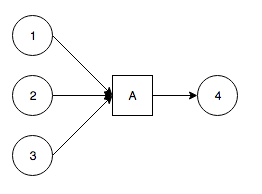
\includegraphics[scale=0.5]{Billeder/HyperEdge.png}
\caption{Example of hyperedge $A$. $T(A) = \{1,2,3\}$, $H(A) = \{4\}$}
\end{figure}

\textbf{Hyperpaths}\\
A path $P_{st}$ from $s$ to $t$ in a B-hypergraph is a sequence $P_{st}=\langle e_1, e_2, e_3, ... , e_q \rangle$ of B-hyperedges such that $s\in T(e_1)$ and $t=H(e_q)$ and $H(e_i) \in T(e_{i+1})$ for $i=1..q-1$. Its length $|P_{st}|$ is the number $q$ of hyperedges. If $t \in T(e_1)$, then $P_{st}$ is a cycle. A hypergraph is acyclic if it does not contain any cycles. \cite{Fagerberg} \\
A hyperpath $\pi_{st} = (V_{\pi},E_{\pi}$ from a source vertex $s$ to a target vertex $t$ in a B-hypergraph $H$ is a subhypergraph of H with the following properties: If $t = s$, the $V_{\pi}=\{s\}$ and $E_{\pi} = \emptyset$. Otherwise, $E_{\pi}$ can be ordered in a sequence $\langle e_1, e_2,....,e_q \rangle$ such that 
\begin{enumerate}
\item 
$T(e_i)\{s\} \cup \{H(e_1),h(e_2,...,h(e_i-1)\}$ for all i
\item
$t=H(e_q)$
\item
Every $v \in V_{\pi} \setminus \{t\} $ has at least one outgoing hyperarc in $E_{\pi}$, and $t$ has zero.
\item
Every $v \in V_{\pi} \setminus \{s\}$ has at least one ingoing hyperarc in $E_{\pi}$, and $s$ has zero. \cite{Fagerberg}
\end{enumerate}

\section{Designing a hypergraph in C++}
A hypergraph consists of nodes and hyperedges. These where implemented as two structs that have their own seperate attributes.
\begin{figure}[H]
\centering
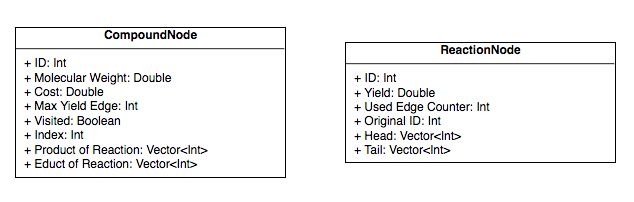
\includegraphics[scale=0.5]{Billeder/Compound-ReactionNode.png}
\caption{The structure of CompoundNodes and ReactionNodes}
\end{figure}
There are some non-trivial attributes in the CompoundNode struct.The difference between Molecular weight and the cost is that the cost is the accumulated weight of the given starting materials that is used to reach this compound, and the molecular weight is the actual weight the compound it self. This of course means that if a compound is a starting compound, then the cost and the molecular weight is the same.\\ The Max Yield Edge attribute is an identifier to the hyperedge that is used to reach this compound. The first time a compound is reached the attribute is changed to hold the ID of the reaction from where the algorithm came. If the compound is reached and the cost of the compound is changed, then the attribute would change, so that it always points to the edge used to calculate the current cost of the compound.\\
Visited and Index are attributes used when the hypergraph is pruned (Section \ref{Pruning}) and to keep track of a CompoundNodes position in the priority queue used when running STB-Dijkstra (Section \ref{STB-Dijkstra}).\\
The two vectors, Product of Reaction and Educt of Reaction, are lists containing information on which reactions the compound is a product of and which reactions it is a educt to. This is used to make traversal of the hypergraph easy.\\

The ReactionNode also contains some non-trivial attributes. The Used Edge Counter is used by the STB-Dijkstra algorithm (Section \ref{STB-Dijkstra}) to make sure that all educts to a reaction have had their min cost evaluated before the reaction can be used. The Original ID attribute is used when we need to change a hyperedge into a B-Hyperedge. If there is more than one product of a reaction we need to split the reaction into multiple new reactions, so that the hyperedge becomes legal. It is for result purpose needed to have a pointer to the original ID of the reaction.\\

The hypergraph is designed to consist of four dynamic lists, vectors, to facilitate quick lookup time and fast attribute reseting. The two vectors compoundList and reactionList are list of size $V$ and $E$ respectively, containing pointers to the compounds and reactions of the given hypergraph. These two vectors are used to reset the attributes of the compounds and reactions after each iteration of the algorithms. The compoundLookupList and reactionLookupList vectors are used to have have a constant lookup time at the cost of space. Both are vectors of pointers to compounds and reactions, just as compoundList and reactionList, but are of size $N$ and $M$ instead, where $N$ is the highest compoundID and $M$ is the highest reactionID. This means that if a reaction with ID 235406 is added to the hypergraph, a pointer to the reaction is pushed to to the back of reactionList and added to reactionLookupList[235406]. This makes it possible to edit a single compound or reaction in $\mathcal{O}(1)$ time, using the lookupLists, and to edit all compounds or reactions in $\mathcal{O}(V)$ and $\mathcal{O}(E)$ respectively.\\
If the structure was only used on homemade hypegraphs where we would label the compounds from $0,1, ... N$ and the reactions $0,1,...,M$, we would only need the two lookupLists, since we would have two vectors of size $V=N$ and $E=M$ and still have the constant lookup time. However, when working on real data we could have a hypergraph with the reactionIDs 6, 12820 and 50003829 as the only reactionsNodes in the hypergraph. This would result in a vector of size 50003829 but we only have three entries in the vector. So when we need to reset the attributes in the use of the shortest path algorithms we would have to run through the whole vector. This is where the two second lists are useful. Even though we have a reactionLookupList of size 50003829 the reactionList in this hypergraph would only be of size 3.
Notice that since we are working with pointers to, and not copies of, compoundNodes or reactionsNodes there is no problem in only changing the attributes by accessing it through one of the lists. 
\begin{figure}[H]
\centering
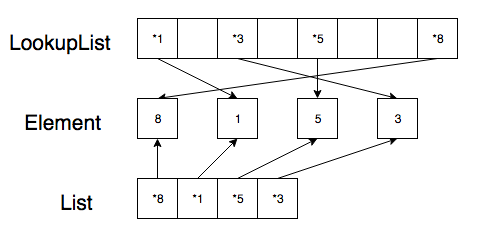
\includegraphics[scale=0.5]{Billeder/ListOverview.png}
\caption{Illustration of the difference between List and LookupList.}
\label{fig::ListLookupList}
\end{figure}
\section{Finding The K-Best Synthetic Plans}
This section describes how to find the K-Best paths of a hypergraph modifying an algorithm made by Jin Y. Yen. The section starts out by describing the work flow of the algorithm, and then proceeds to deal with the alterations that are needed to run the algorithm on a hypergraph.
\subsection{Yen's Algorithm}
Yen's algorithm is an algorithm that computes the K-shortest paths for a graph with non-negative edges. It was publish in 1971 and uses any shortest path algorithm to find the best path and then proceeds to find the $K-1$ deviation of the best path. \cite{Yen}

It starts out by finding the best path using a shortest path algorithm. Once the best path have been found it uses the path to find all the potential second best paths by fixing and removing edges in the graph. \\
By using the same first vertex as the original path but removing the first edge, it forces the shortest path algorithm to take another route through the graph and thereby creating a potential second best path. This is added to the list of potential paths and the algorithm can continue to derive other paths from the best path. By fixing the first edge in the previous best plan, Yen's algorithm forces the shortest path algorithm to take the first edge which it now shares with the best path. However, now the algorithm have removed the second edge from the original path and once again forces the shortest path algorithm to find alternative routes. This process is then repeated until we reach the next to last vertex in the best path.\\
By sorting the list of potential paths, it has the second best path at the start of the list and it can add it to the final list of best path. The algorithm then repeats on the second best path to find the third best path. This is done until all K-best path have been found or there are no more paths to find.
\subsection{Yen's Algorithm On Hypergraphs}
We use the principles from Yen's algorithm to make our own algorithm that will work on hypergraphs. To handle the problem of generating all derived paths from our best path in our hypergraph, we use a method called BackwardsBranching. \cite{Fagerberg} \cite{Nielsen} \cite{Carsten}
\begin{lstlisting} [emph={if,for, endif, endfor, function, endfunction, do}, emphstyle = \bfseries,caption = Backwards Branching for B-Hypergraph]
function Back-Branch(H,$\pi$)
	B=$\emptyset$
	for i = 1 to q do 
		Let H$^i$ be a new hypergraph
		H$^i$.V = H.V
		// Remove hyperarc from H
		H$^i$.E = H.E $\setminus \{\pi.p(v_i)\}$
		// Fix Back tree
		for j = i+1 to q do
			H$^i$.BS(vj) = \{$\pi.p(v_j)$\}
		B = B $\cup$ \{H$^i$\}
	return B
\end{lstlisting}
\begin{figure}[H]
\hspace{-2cm}
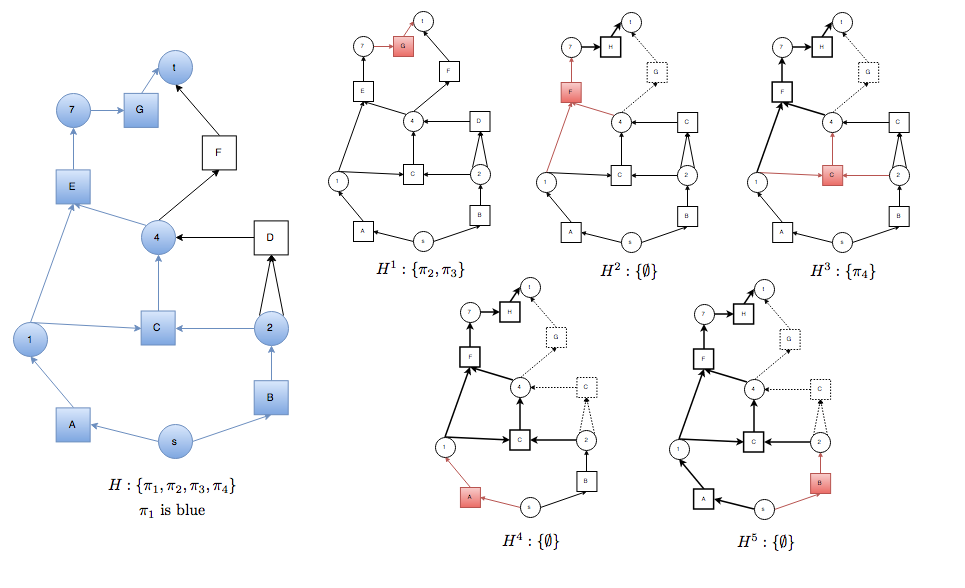
\includegraphics[scale=0.5]{Billeder/BachBranch}
\caption{An example of branching for hypergraphs. $H$ is the original hypergraph. The vertices and hyperedges marked with blue are part of the best path. The rest of the figure illustrates the backwards branching. Each of the smaller figures shows a hypergraph $H^i$ and how it is created from $H$. Dotted hyperedges and red heyperedges are not part of the hypergraph, but have been deleted due to branching. Hyperedges in bold are fixed hyperedges. When hyperedges are fixed it leads to other hyperedges being deleted (dotted). The caption beneath each hypergraph represents the possible paths that are available in the given hypergraph.}
\end{figure}
However, this algorithm have a problem when working on a larger hypergraph. It demands that each time we make alterations on the hypergraph we have to make a copy, $H^i$, of the graph, $H$, with the exception of the hyperedges that is removed when fixing the back tree and removing $\pi.p(v_i)$.\\
This could easily work for smaller graphs, but if we use this on the hypergraph that we generate from the beilstein database, we would have to copy a graph of multiple GigaBytes. \\
To handle this problem I came up with the idea of creating an overlay for the graph instead of copying it. The overlay would work as an transparent on top of the original graph, stating which edges still is accessible. This is done by creating a \textit{vector<bool>} which has a length of $R$, where $R$ is the number of reactions. Normally a reaction would contain at least 28 bytes of data:
\begin{itemize}
\item
3x ints of 4 bytes each
\item
1x double of 8 bytes
\item
1x \textit{vector<int>} head of length one of at least 4 bytes
\item
1x \textit{vector<int>} tail of length $N$ (number of educts) of at least 4 bytes
\end{itemize}
This can be reduced dramaticly by using the \textit{vector<bool>}, since c++ only uses 1 bit per boolean in the vector instead of the regular 1 byte per boolean.\cite{VectorBool} This means if working on a hypergraph with 40 million reactions, we would be able to create an overlay using 5 MB of space per alternated graph, instead of copying a hypergraph were the reactions alone uses at least 1,12 GB per copy. \\
As the figure below shows, we never change or remove anything on the hypergraph. We simply create the following overlay:
\begin{table}[H]
\centering
\begin{tabular}{c|c|c|c|c}
Reaction & A & B & C & D \\\hline
Usable & true & true & true & false \\\hline
Bit Representation & 1 & 1 & 1 & 0
\end{tabular}
\end{table} 
And then when trying to use an edge, we ask: "Does overlay at reaction A exist?". If yes, you can use it. If no, the edge have been "removed", and therefore cannot be used.
\begin{figure}[H]
\centering
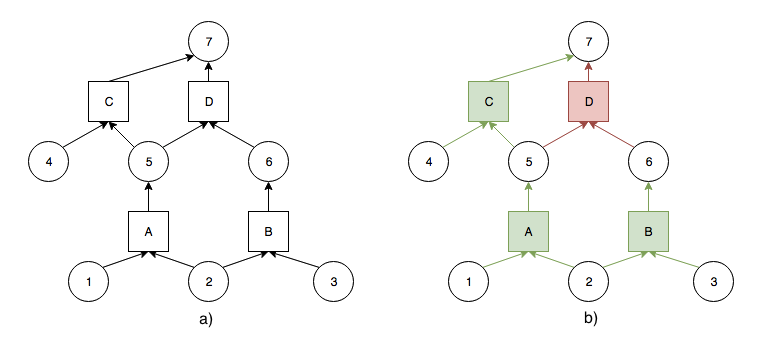
\includegraphics[scale=0.5]{Billeder/OverlayIllustration}
\caption{a) The original hypergraph. b) The original hypergraph, but using the overlay. If the reaction is green it is still usable. If red then it have been "removed" from the hypergraph.}
\end{figure}

This of course means that the algorithm for back-branch have to be changed accordingly. Instead of the hypergraph as input we now give it an overlay. This overlay is changed so it fits with the new layout of the graph. Instead of deleting hyperedges in the copy, we now simply changes the boolean at the index of the hyperedge.id. True if we should "add" the hyperedge and false when we want to "remove" a hyperedge.

\begin{lstlisting} [emph={if,for, endif, endfor, function, endfunction, do}, emphstyle = \bfseries,caption = Backwards Branching for B-Hypergraph using overlay]
function BackwardsBranching($\pi$, Overlay) 						
	List B = $\emptyset$
	// q = Path length
	for i = 1 to q do			
		//remove i'th hyperedge from Path in overlay					
		Set Overlay[$\pi$[i]] to false		
		//fix the backtree				
		for j = i downto 1	do							
			vertex C <- $\pi$[j].head
			for each hyperedge into C
				Set Overlay[reaction.id] to false
			Set Overlay[$\pi$[j]] to true
		endfor
		B = B $\cup $ {$Overlay$}
	endfor
	return B
endfunction
\end{lstlisting}
Now that we have the branching in place are we able to construct an algorithm that are similar to Yen's algorithm, but can run on hypergraphs. As input it takes a start node ($s$), a goal node ($t$), and an integer $K$, where $K$ is the number of best paths we want to find. The algorithm, however, only takes a single node as its starting node, which is a problem when working with hypergraphs. The reason for this is that the size of the tail of a hyperedge usually is larger than 1 and this by default gives us more than one starting node. This is fixed by making $s$ a dummy node that have an hyperedge $e = (H|1|, T|1|)$ to each of the starting nodes, transforming the multiple sources to a single source.\\
The algorithm creates a heap, $L$, and a list, $A$, which will contain the $K$-best paths once the algorithm is finished. It then finds the best path using a shortest path algorithm and inserts it into the heap. Inside the loop it extracts the best path found from the heap and performs a backward branching, and finds all possible paths in the branches. If there is a path from $s$ to $t$, then this path is added to the heap. The algorithm either terminates if the heaps is empty ( No more paths available) or once it have found the $K$-best paths.
\begin{lstlisting} [emph={if,for, endif, endfor, function, endfunction, do}, emphstyle = \bfseries,caption = K-Shortest Paths Algorithm in B-Hypergraph]
function YenHyp(s, t, K) 
	L = new heap with elements (overlay, $\pi$)
	A = List of shortest paths
	//(Graph is default overlay (all true))
	$\pi$ = shortestPath(Graph, s,t) 				
	Insert (Graph, $\pi$) into L
	for k = 1 to K do
		if L = $\emptyset$
			Break
		endif
		(Overlay$'$, $\pi'$) = L.pop
		add $\pi'$ to A
		for all Overlay$^i$ in BackwardBranching((Overlay$'$,$\pi'$)) do
			$\pi^i$ = shortestPath(Overlay$^i$, s, t)
			if $\pi^i$ is complete
				Insert( $H^i$, $\pi^i$) into L
			endif
		endfor
	endfor
	return A
endfunction
\end{lstlisting}
YenHyp makes $K$ iterations. In each iteration the length of a hyperpath determines the number of calls to the shortest path algorithm. The worst case for the length of the hyperpath is $\mathcal{O}(|V|)$. Hence the running time of YenHyp becomes:
\begin{equation}
\mathcal{O}(K \cdot |V| \cdot SP)
\end{equation}
Where $SP$ is the running time for the shortest path algorithm used.
\subsection{Cost Function}
Before we are able to find the K-best paths of our hypergraph, we should be able to compare them with each other. To do this we use a additive weight function defined in the following way on a given hyperpath $\pi_{st}$ from $s$ to $t$:

\begin{equation}
W(u)=\begin{cases}
    w(p(u)) + F(p(u)), & \text{if $u\in V\setminus \{s,\ starting\ nodes\}$}.\\
    C, & \text{Starting Nodes}. \\
    0, & \text{Otherwise}
  \end{cases}
\end{equation}

$W(u)$ define the cost of node $u$ and $C$ is in this particular case, the molecular weight of a compound. The predecessor function $p$ is used to find the hyperedge $e=p(u)$ which have $u$ as head. The function $F$ is a non-decreasing function of the sum of the weights of the nodes in the tail to $e$. Each of the nodes are multiplied by the retroyield of the edge, $1/yield$.

\begin{equation}
F(p(u)) = \sum(W(Tail(p(u)) \cdot (1/yield_{p(u)})
\end{equation}

We are now able to distinguish between the paths found and extract the K-best plans. \cite{Carsten}

\section{Shortest Path}
This section describes two different approaches to the shortest path problem in a hypergraph. A dynamic approach proposed by Carsten Grønbjerg Lützen and Daniel Fentz Johansen \cite{Carsten} and a Dijkstra inspired approach proposed by Lars Relund Nielsen, Kim Allan Andersen and Daniele Pretolani \cite{Nielsen}. 

\subsection{Dynamic Approach}
kkk \cite{Carsten}\\
kkkk \cite{Fagerberg}\\

\subsubsection{Approach}
\begin{lstlisting} [emph={if,for, endif, endfor, function, endfunction, do}, emphstyle = \bfseries,caption = Dynamic programming for finding the best path]
function Min(V)
	if(V) is starting material 
		return Cost of V
	endif
	mincost <- $\inf$
	for all $e\in BS(V)$ do
		cost <- cost of e
		for all $u \in Tail(e)$ do
			cost <- cost + Min(u)
		endfor
		if mincost $\leq$ cost 
			mincost <- cost
			V.minedge <- e
		endif
	endfor
	return mincost
endfunction
\end{lstlisting}

$\mathcal{O}(V+E)$


\subsubsection{Problems}
A problem with the dynamic approach is that it does not work on hypergraphs with cycles due to its recursive nature. When a cycle it hit, it will start an endless loop to figure out the cost of a node. 
\begin{figure}[H]
\centering
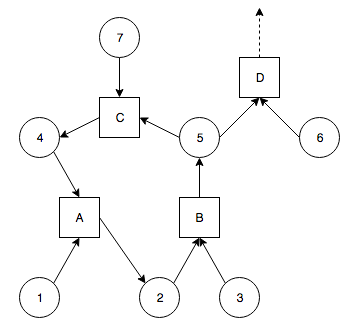
\includegraphics[scale=0.5]{Billeder/CycleGraph.png}
\caption{Example of graph with cycle.}
\label{fig::CycleGraph}
\end{figure}
As seen in the example in fig. \ref{fig::CycleGraph}, the algorithm enters the cycle in reaction D. When trying to calculate the weight of 5, it needs the weight of 2 and 3. 3 is a starting node, so the weight is the weight of the compound itself. 2 however needs the weight of 1 and 4. Again 1 is a starting node, so no calculations are needed. 4 however needs the weight from 7 and 5. Now we hit 5 again, and the loop starts. This could of course be handled by removing an edge from  the hypergraph, and thereby breaking the cycle. This however would effect the results, because how do we know that the edge we remove would not have contributed to a better result in the end. This is where Nielsen et. el STB-Dijkstra algorithm comes into play.
\subsection{The STB-Dijkstra Algorithm} \label{STB-Dijkstra}
Nielsen algorithm, or SBT-Dijkstra, is an algorithm that uses the same principles as shortest path algorithm conceived by Edsger W. Dijkstra in 1956. The original Dijkstra is asymptotically the fastest known single-source shortest-path algorithm for arbitrary directed graphs with unbounded non-negative weights. \cite{Dijkstra} Nielsen et. al. have modified it to be used on hypergraphs.
\subsubsection{Approach}
The algorithm requires that the cost of all nodes in the hypergraph is $\infty$ and that the hyperedge property $kj=0$. It then adds the dummy node $s$ to its priority queue. As long as the priority queue is not empty it will extract the minimum, and for each hyperedge going out of $u$ increase the $kj$ counter in the given hyperedge. Once the counter is equal to the size of the tail of the hyperedge, the algorithm can proceed to calculate the weight of the node $v$, which is the head of the hyperedge. Should the existing weight of $v$ be larger than the newly calculated weight, the algorithm updates the weight to the newly found weight and adds $v$ to the priority queue, given that the node have not been added from another edge. If the cost changes, the min-edge attribute is also set to be the edge from which the new cost have been calculated.
\begin{lstlisting} [emph={if,for, endif, while, endwhile, endfor, function, endfunction, do}, emphstyle = \bfseries,caption = STB-Dijkstra for finding the best path]
Initialization: Set W(u) = $\infty \ \forall\ u \in V$, $k_j = 0\ \forall\ e_j \in E$,$Q = \{s\}$ and $W(s)=0$
function SBT-Dijkstra
	while ($Q=\emptyset$) do
		select and remove $u\in Q$ such that $W(u) = min\{W(x)|x\in Q\}$
		for ($e_j \in FS(u)$) do
			$k_j <- kj+1$
			if ($k_j = |T(e_j)|$) 
				v <- h($e_j$)
				if (W(v) > w($e_j$) + F($e_j$))
					if ($v \notin Q$  
						Q <- Q $\cup$ \{v\}
					endif
					W(v) <- w($e_j$)+ F($e_j$)
					p(v) <- $e_j$
				endif
			endif
		endfor
	endwhile
endfunction
\end{lstlisting}
When node $u$ is removed from the candidate set $Q$ (the priority queue), $W(u)$ is the minimum weight of all hyperpath from $s$ to $u$. The condition in line 7 ensures that each hyperedge $e_j$ is processed only once after the minimum cost for its tail nodes have been determined. The implementation of the priority queue, $Q$, dictates the running time of the algorithm. I have followed Nielsen et. al. example and chosen a heap structure. Since I have decided to implement the simple binary heap the running time of the algorithm becomes: $\mathcal{O}(E\ log_2(V) + size(h))$. The size of the hypergraph, $h$, is the sum of the cardinalities of its hyperedges:

\begin{equation}
size(h) = \displaystyle\sum_{e\in E} |e|.
\end{equation}
Where the cardinality of a hyperedge $e$ is the number of nodes it contains, i.e. $|e| = |T(e)| + 1$.\cite{Nielsen}
\subsubsection{Optimizing For Large Hypergraphs}\label{Pruning}
Since the STB-Dijkstra algorithm expands to the whole graph it might check nodes that is not a part of the hyperpath we are looking for. If we look at the hypergraph in fig. \ref{fig::DeadEnd}, is it easy to see that given the starting nodes 1,2,3,4 and the goal 10, that there is no need to use the hyperedges R2, R4, and R8, since they never would lead to our goal.
\begin{figure}[H]
\centering
\includegraphics[scale=0.4]{Billeder/DeadEnd.pdf}
\caption{}
\label{fig::DeadEnd}
\end{figure}

I therefore decided to combine the dynamic approach with STB-Dijkstra algorithm. The dynamic approach starts at the goal node, and travel through the hypergraph until it reaches $s$, thereby only using nodes on the way from goal to start. The algorithm however had the problem of not being able to work on hypergraphs that contained a cycle, and we could not just delete an edge when we hit a cycle since it could lead to wrong results.\\
We can however use the dynamic algorithm to mark the edges it hits on the way from goal to start. This would make it able to detect when it hits a cycle, since the node would already have been marked, and simply just skip the node and proceed to the next in its potential path. Once the algorithm is finished, we can transform the markings to an overlay that limits the hypergraph so it only "consist" of the reactions hit by the dynamic algorithm. Using this overlay reduces the search space of the STB-Dijkstra from the whole hypergraph to only concern the hyperedges that will lead to a path from $s$ to $t$.
\begin{lstlisting} [emph={if,for, endif, while, endwhile, endfor, function, endfunction, do}, emphstyle = \bfseries,caption = Reduce STB-Dijkstra search space]
graphOverlay is a list of size = #hyperedges where all entries are false.
function reduceGraph(graphOverlay, v, s)
	if (v.id = s.id)
		return graphOverlay;
	endif
	if (v.visited = false) 
		for(reaction : v.ingoingEdge )
			for (tailCompound : reaction->tail) 
				v.visited <- true;
				graphOverlay = reduceGraph(graphOverlay, tailCompound, s);
			endfor
			graphOverlay[reaction.id] <- true;
		endfor
	endif
	return graphOverlay;
\end{lstlisting}
Since the running time for the dynamic approach was $\mathcal{O}(V+E)$, the combined running time becomes: 
\begin{equation}
\mathcal{O}((V+E)+(E\ log_2 (V) + size(h)))
\end{equation}
The $(V+E)$ is however removed since the $E\ log_2 (V) + size(h)$ dominates. This results in a running time of:
\begin{equation}
\mathcal{O}(E\ log_2 (V) + size(h))
\end{equation}
The reason that the terms $V$ and $E$ does not change since in worst case are we not able to prune any of the hypergraph away using the dynamic approach.
\subsection{Testing}
Rojin tests - using Carstens Synthworker. 
\section{Beilstein Data}
The Beilstein database is the largest database in the field of organic chemistry. Since 2009, the content has been maintained and distributed by Elsevier Information Systems in Frankfurt under the name "Reaxys".
The content covers more than 200 years of chemistry and has been abstracted from several thousands of journal titles, books and patents. Today the data is drawn from selected journals (400 titles) and chemistry patents, and the extraction process for each reaction or substance data included needs to meet three conditions:
\begin{enumerate}
\item
It has a chemical structure
\item
It is supported by an experimental fact (property, preparation, reaction)
\item
It has a credible citation
\end{enumerate}
Journals covered include \textit{Advanced Synthesis and Catalysis, Angewandte Chemie, Journal of American Chemical Society, Journal of Organometallic Chemistry, Synlett} and \textit{Tetrahedron}. \cite{WikiReaxys}\cite{WikiBeilstein}
\subsection{Data Assessment}
During my work with the Beilstein database have I found several issues when it comes to using it to find shortest paths.
First problem is that there are multiple instances of the same compound, each with a different Reaxys IDs. As seen in fig.\ref{fig::SameID} have I found four different IDs for the compound Dysidiolide. These were found when I tried to reproduce the different synthesis plans of Dysidiolide from \cite{SynthesisPlans} using the referenced articles where each synthesis plan origins. E. J. Corey's version of Dysidiolide have the ID 8171938, Boukouvalas have two different with ID 7601810 and 7910427 and Danishefsky have the ID 7910428. \\
Since we have four different IDs for Dysidiolide we can't state a single goal compound to our program that would result in giving us these three synthesis plans. To handle this problem the program can take several goal compounds as an input, and by creating a dummy node $t$ are we able to give the illusion of a single target.

\begin{figure}[H]
\hspace{-1cm}
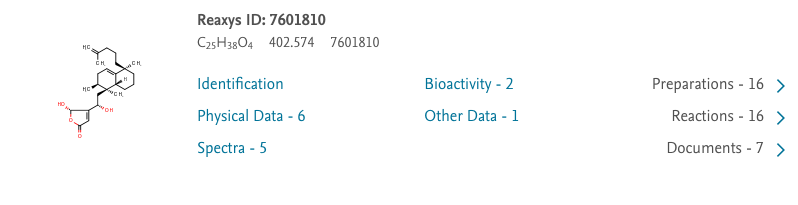
\includegraphics[scale=0.5]{Billeder/Dysidiolide-7601810.png}

\hspace{-1cm}
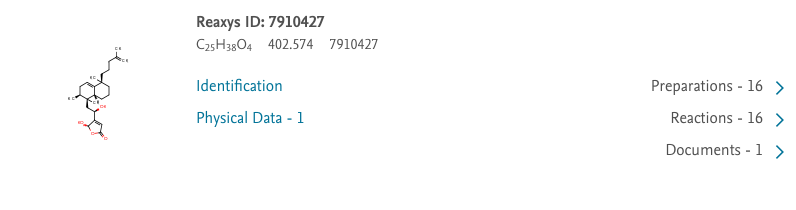
\includegraphics[scale=0.5]{Billeder/Dysidiolide-7910427.png}

\hspace{-1cm}
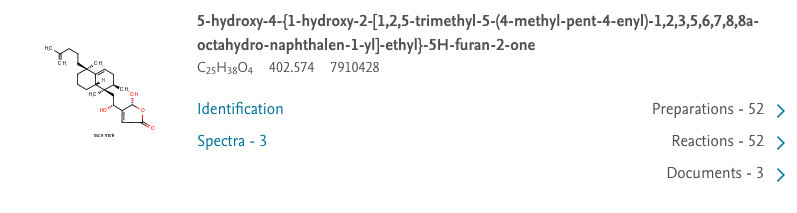
\includegraphics[scale=0.5]{Billeder/Dysidiolide-7910428.png}

\hspace{-1cm}
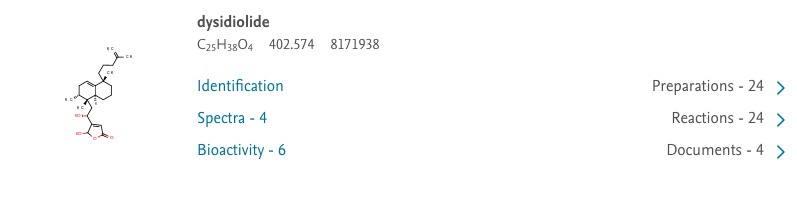
\includegraphics[scale=0.5]{Billeder/Dysidiolide-8171938.png}
\caption{Four different instances of Dysidiolide in Reaxys.}
\label{fig::SameID}
\end{figure}

So what is causing this multiple ID issue? If we study fig. \ref{fig::SameID} can we see that the molecular weight and molecular formular are exactly the same, however if we look at the close up of the molecular structure in fig. \ref{fig::SameIDClose} the compounds are not structured in the same way, even though the compounds are the same. The main differences is:
\begin{enumerate}
\item
Which way some of the substructures are facing. Example: The lower $C_4O_3H_4$ is rotated differently in each instance or that we write $H_2C$ instead of $CH_2$.
\item
How the bond between two chemical elements are notated. Example: The bond to the $OH$ in the bottom of the structure is either a "single" (d), "single down" (a) (c) or "single up or down" (b).
\end{enumerate}

\begin{figure}[H]
\begin{subfigure}{.5\textwidth}
  \centering
  \vspace{0.4cm}
  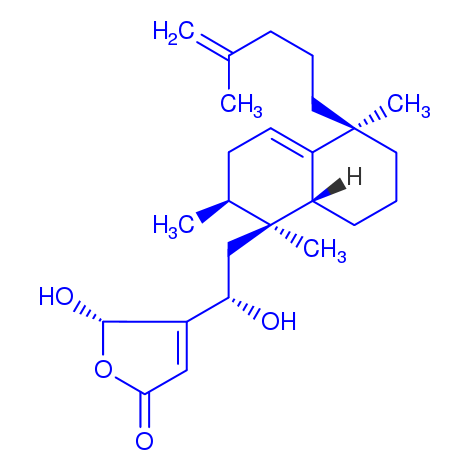
\includegraphics[width=.8\linewidth]{Billeder/Dysidiolide-7601810-Close.png}
  \vspace{1.3cm}
  \caption{}
\end{subfigure}%
\begin{subfigure}{.5\textwidth}
  \centering
  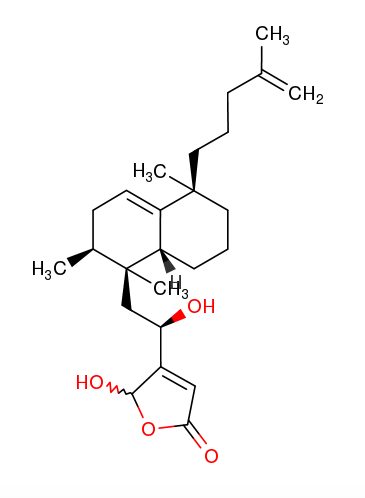
\includegraphics[width=.8\linewidth]{Billeder/Dysidiolide-7910427-Close.png}
  \caption{}
\end{subfigure}
\begin{subfigure}{.5\textwidth}
  \centering
  \vspace{0.4cm}
  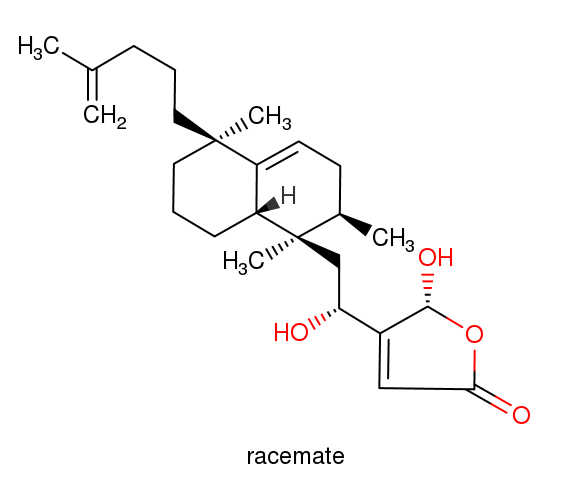
\includegraphics[width=.8\linewidth]{Billeder/Dysidiolide-7910428-Close.png}
  \vspace{1.3cm}
  \caption{}
\end{subfigure}%
\begin{subfigure}{.5\textwidth}
  \centering
  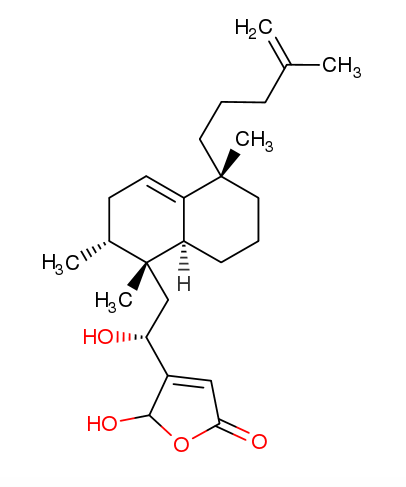
\includegraphics[width=.8\linewidth]{Billeder/Dysidiolide-8171938-Close.png}
  \caption{}
\end{subfigure}
\caption{Different versions of Dysidiolide: (a) ID 7601810 , (b) ID 7910427, (c) ID 7910428,  (d) ID 8171938}
\label{fig::SameIDClose}
\end{figure}

Second issue is the problem of a reaction not having an educt or a product(fig: \ref{fig::EductProductMissing}). This leaves the reaction incomplete and makes it useless in the graph construction. If there is no educt the hyperedge created will have an indegree of 0, and thereby making it unreachable. If there is no product the hyperedge will have an outdegree of 0, making it a deadend.

\begin{figure}[H]
\hspace{-1cm}
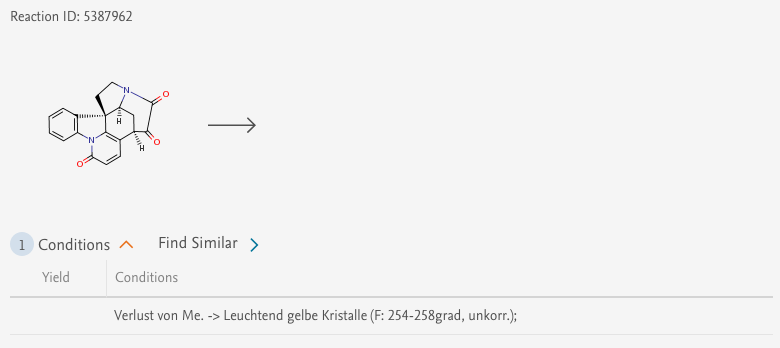
\includegraphics[scale=0.5]{Billeder/LeftOnlyReaction.png}

\hspace{-1cm}
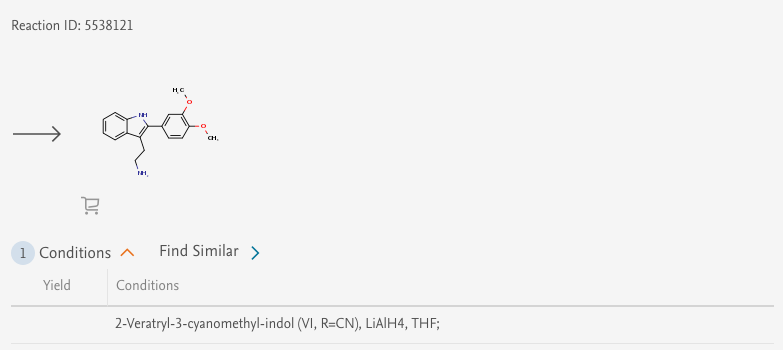
\includegraphics[scale=0.5]{Billeder/RightOnlyReaction.png}
\caption{Example of reactions that either is missing educts or products.}
\label{fig::EductProductMissing}
\end{figure}

Third issue is that some reactions contains educts where a compound isn't linked to a compound in the database. This results that the name of the compound is written instead of the usual structure diagram (fig \ref{fig::NoCompound}). This issue does not give problems when it comes to the construction of the hypergraph. The compound is simply just not added to the hypergraph. This however results in a slightly misleading result if the user does not look up the reaction in Reaxys where the name of the educt is stated. Example: If $A+B\rightarrow C$ but $B$ is not given an compound ID the reaction would look like $A\rightarrow C$ in the hypergraph.

\begin{figure}[H]
\hspace{-1cm}
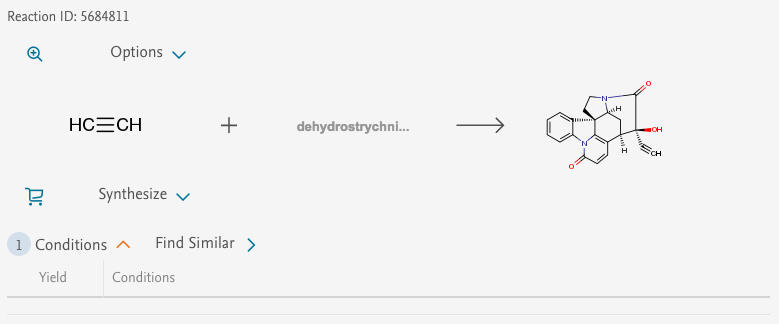
\includegraphics[scale=0.5]{Billeder/MissingIngredientReaction.png}
\caption{Example of an reaction with a missing educt.}
\label{fig::NoCompound}
\end{figure}

Forth issue is multireactions. (fig \ref{fig::Multistep}) A mulitreaction is a reaction with its own ID, but it consists of an educt and a product were there are multiple reaction steps, $s$, between the two compounds. This means that instead of $s$ different reactions with their own ID and yield we get a single reaction without a yield. The yield for each reaction in the multistep reaction is often stored as a part of the reaction text, but not easy extractable. The multistep reaction should however only consist of individual reactions that already are in the database.\\
The solution to this problem have been to not include all reactions labelled as "Multi-step reaction" to the extraction from the database. Since the steps should be saved as individual reactions this would not cause any harm to possibility of finding the exact same path, but only using all $s$ steps instead of one.

\begin{figure}[H]
\hspace{-1cm}
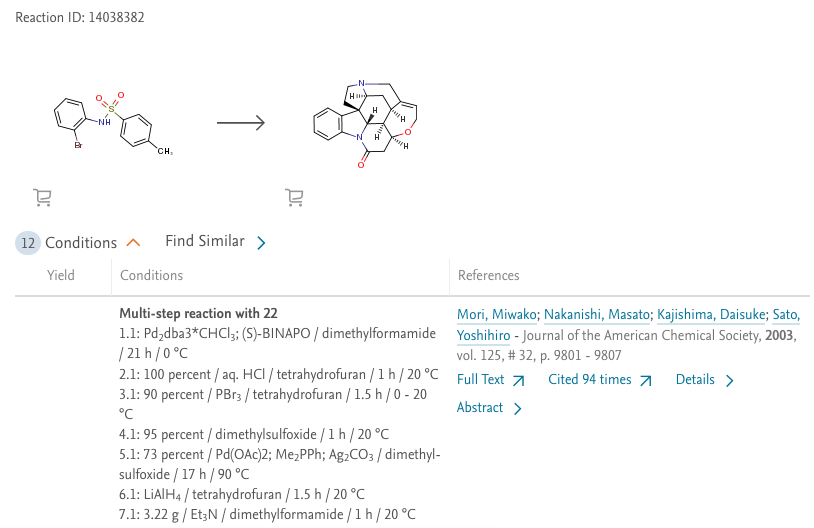
\includegraphics[scale=0.5]{Billeder/MultistepReactions.png}
\caption{Example of a multistep reaction.}
\label{fig::Multistep}
\end{figure}

\begin{figure}[H]
\hspace{-1cm}
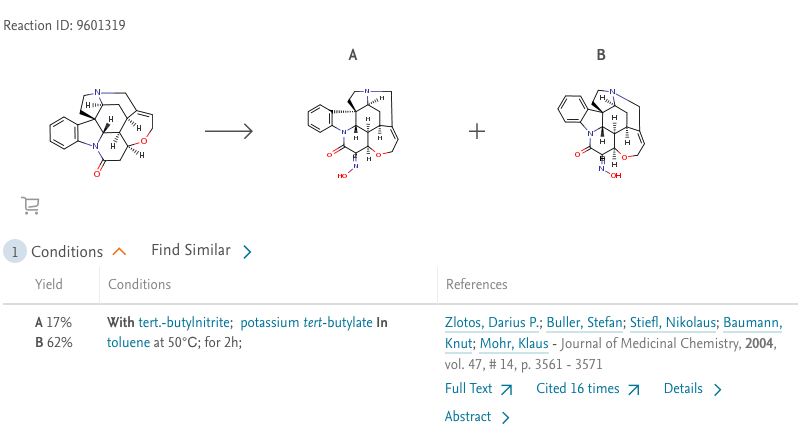
\includegraphics[scale=0.5]{Billeder/MultipleProducts.png}
\caption{Example of a reaction with multiple products}
\label{fig::MultipleProducts}
\end{figure}
\label{ConvertToB-Hypergraph}
Fifth issue is reactions which have more than one product (fig. \ref{fig::MultipleProducts}). If this becomes a part of our hypergraph it is no longer a B-hypergraph. This is a problem since both shortest paths algorithms only works on B-hypergraphs. This problem is however solved after the graph have been created by the method $convertToBHypergraph()$ in Hypergraph.hpp. The method iterates through the reaction list and if it encounters a non B-hyperedge, the hyperedge is added to a list of non B-hyperedges. For each of the non fixed B-hyperedges ,$e$, it creates $|H(e)|$ new hyperedges ,$e_i$, where $T(e_i)=T(e)$ and $H(e_i) = H(e)[i], \forall\ i \in \mathbb{N}, 1 \leq i\leq|H(e)|$  (fig. \ref{fig::CopyReaction}). Each of the new reactions contains an original-ID variable that points to the original hyperedge. This is only used to print the correct ID when the edge is used in a synthesis plan.

\begin{figure}[H]
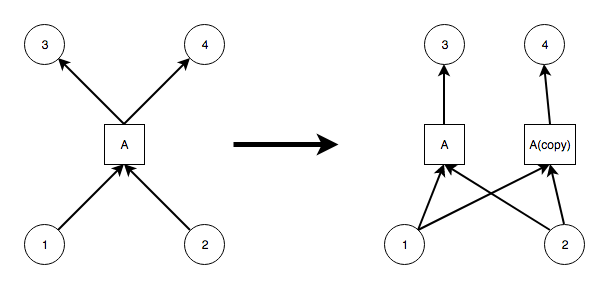
\includegraphics[scale=0.5]{Billeder/CopyReaction.png}
\caption{Convertion to B-Hyperedge}
\label{fig::CopyReaction}
\end{figure}

\section{Results}
\subsection{Pre-work}
\subsection{Strychnine}
\begin{table}[H]
\centering
\begin{tabular}{|r|r|r|}
\hline
Plan & Reactions & Starting weight \\ \hline
1 & \ref{Appendix::Strychnine1} & 2471,93 \\\hline
2 & \ref{Appendix::Strychnine2} & 3941,73 \\\hline
3 & \ref{Appendix::Strychnine3} & 4577,65 \\\hline
4 & \ref{Appendix::Strychnine4} & 5871,33 \\\hline
5 & \ref{Appendix::Strychnine5} & 6076,83 \\\hline
6 & \ref{Appendix::Strychnine6} & 8186,61 \\\hline
7 & \ref{Appendix::Strychnine7} & 8558,73 \\\hline
8 & \ref{Appendix::Strychnine8} & 13054,3 \\\hline
9 & \ref{Appendix::Strychnine9} & 13647,7 \\\hline
10 & \ref{Appendix::Strychnine10} & 19444,8 \\\hline
11 & \ref{Appendix::Strychnine11} & 20125,4 \\\hline
12 & \ref{Appendix::Strychnine12} & 20328,7 \\\hline
13 & \ref{Appendix::Strychnine13} & 21040,2 \\\hline
14 & \ref{Appendix::Strychnine14} & 21587,3 \\\hline
15 & \ref{Appendix::Strychnine15} & 44400,5 \\\hline
16 & \ref{Appendix::Strychnine16} & 277503 \\\hline

\end{tabular}
\end{table}

\subsection{Colchicine} 
\begin{table}[H]
\centering
\begin{tabular}{|r|r|r|}
\hline
Plan & Reactions & Starting weight \\ \hline
1 & \ref{Appendix::Colchicine1} & 1719,6 \\\hline
2 & \ref{Appendix::Colchicine2} & 3373,05 \\\hline
3 & \ref{Appendix::Colchicine3} & 50401,9 \\\hline
4 & \ref{Appendix::Colchicine4} & 119547 \\\hline
5 & \ref{Appendix::Colchicine5} & 136227 \\\hline
\end{tabular}
\end{table}

\subsection{Dysidiolide}
\begin{table}[H]
\centering
\begin{tabular}{|r|r|r|}
\hline
Plan & Reactions & Starting weight \\ \hline
1 & \ref{Appendix::Dysidiolide1} & 6801,04 \\\hline
2 & \ref{Appendix::Dysidiolide2} & 8647,76 \\\hline
3 & \ref{Appendix::Dysidiolide3} & 10080,6 \\\hline
4 & \ref{Appendix::Dysidiolide4} & 12385,7 \\\hline
5 & \ref{Appendix::Dysidiolide5} & 12729 \\\hline
6 & \ref{Appendix::Dysidiolide6} & 15597,5 \\\hline
7 & \ref{Appendix::Dysidiolide7} & 21165,7 \\\hline
8 & \ref{Appendix::Dysidiolide8} & 22294,4 \\\hline
9 & \ref{Appendix::Dysidiolide9} & 23259 \\\hline
10 & \ref{Appendix::Dysidiolide10} & 27928,3 \\\hline
\end{tabular}
\end{table}

\subsection{Asteriscanolide}
\begin{table}[H]
\centering
\begin{tabular}{|r|r|r|}
\hline
Plan & Reactions & Starting weight \\ \hline
1 & \ref{Appendix::Asteriscanolide1} & 649,346 \\\hline
2 & \ref{Appendix::Asteriscanolide2} & 5175,63 \\\hline
3 & \ref{Appendix::Asteriscanolide3} & 13549,2 \\\hline
\end{tabular}
\end{table}

\subsection{Lepadiformine}
\begin{table}[H]
\centering
\begin{tabular}{|r|r|r|}
\hline
Plan & Reactions & Starting weight \\ \hline
1 & \ref{Appendix::Lepadiformine1} & 841,29 \\\hline
2 & \ref{Appendix::Lepadiformine2} & 1061,41 \\\hline
3 & \ref{Appendix::Lepadiformine3} & 1129,16 \\\hline
4 & \ref{Appendix::Lepadiformine4} & 5138,44 \\\hline
5 & \ref{Appendix::Lepadiformine5} & 7629,88 \\\hline
6 & \ref{Appendix::Lepadiformine6} & 8116,89 \\\hline
\end{tabular}
\end{table}

kkkk \cite{SynthesisPlans}\\

\section{Further work}
Expand from compounds - making all nodes with indegree 0 as starting compounds - expand from existing plans - generating new synthesis based on already known reactions.
\section{Conclusion}

\newpage

\printbibliography[type=book, title={Books}]
\printbibliography[type=article, title={Articles}]
\printbibliography[nottype=book, nottype=article, title={Other}]

\newpage
\appendix
\addtocontents{toc}{\protect\setcounter{tocdepth}{0}}

\section{Synthesis plans}
\subsection{Strychnine plan 1}
\centering
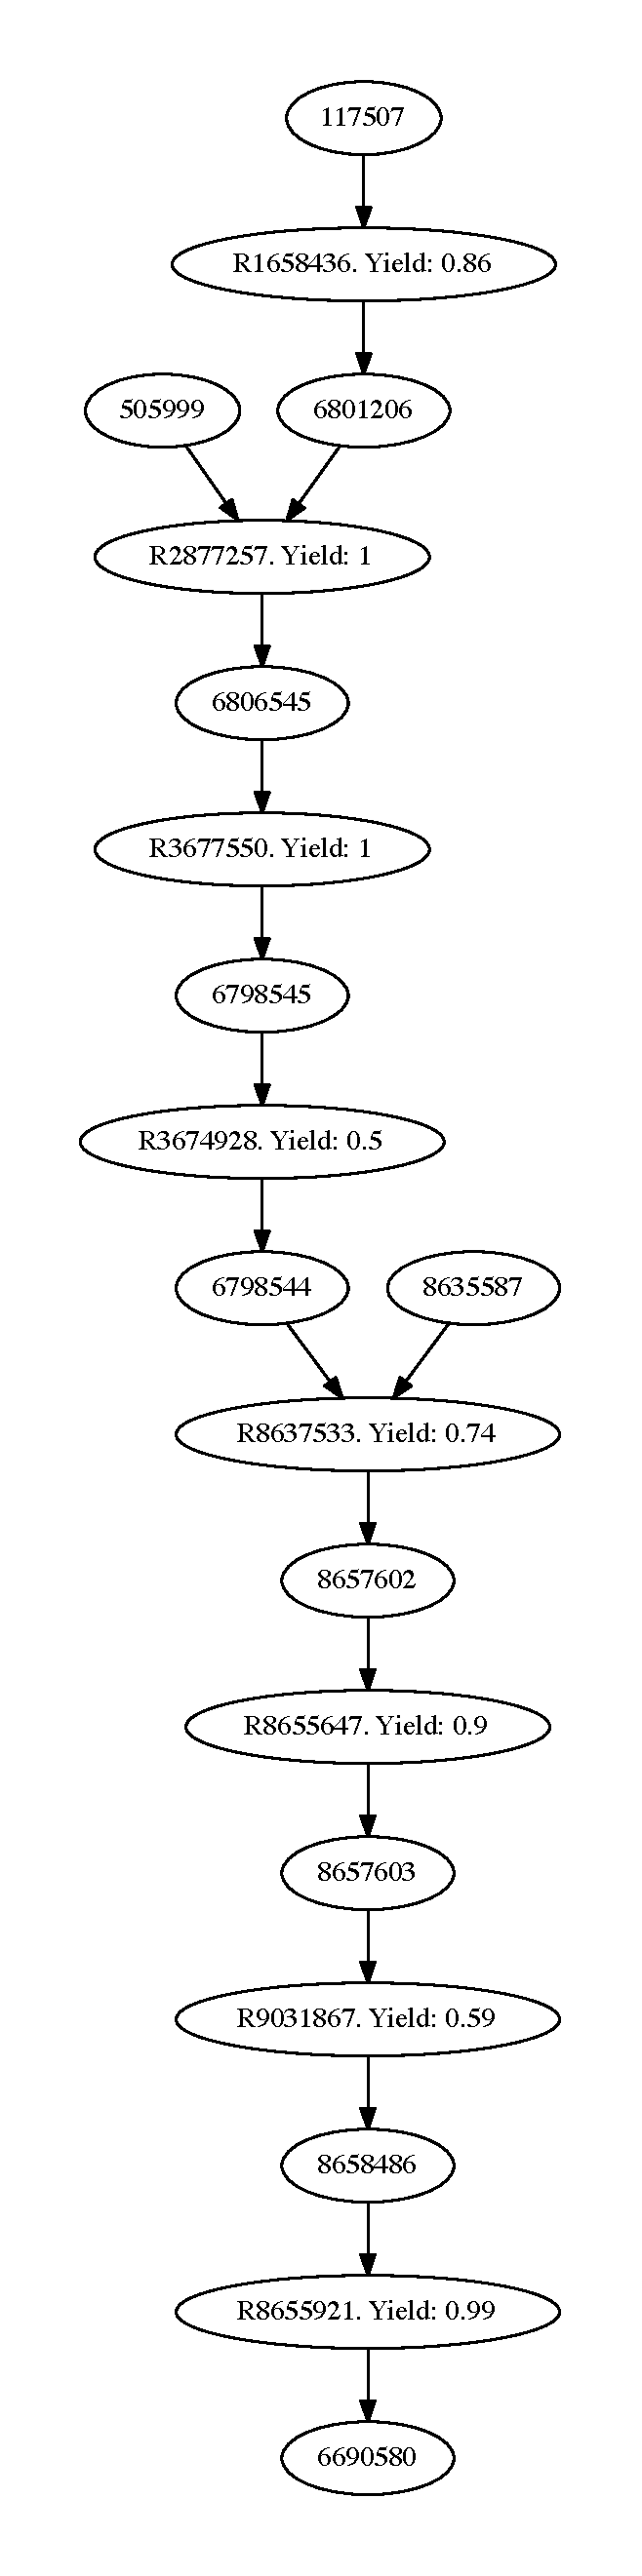
\includegraphics[scale=0.4]{Synteseplaner/Strychnine/plan1.pdf}
\label{Appendix::Strychnine1}

\subsection{Strychnine plan 2}
\centering
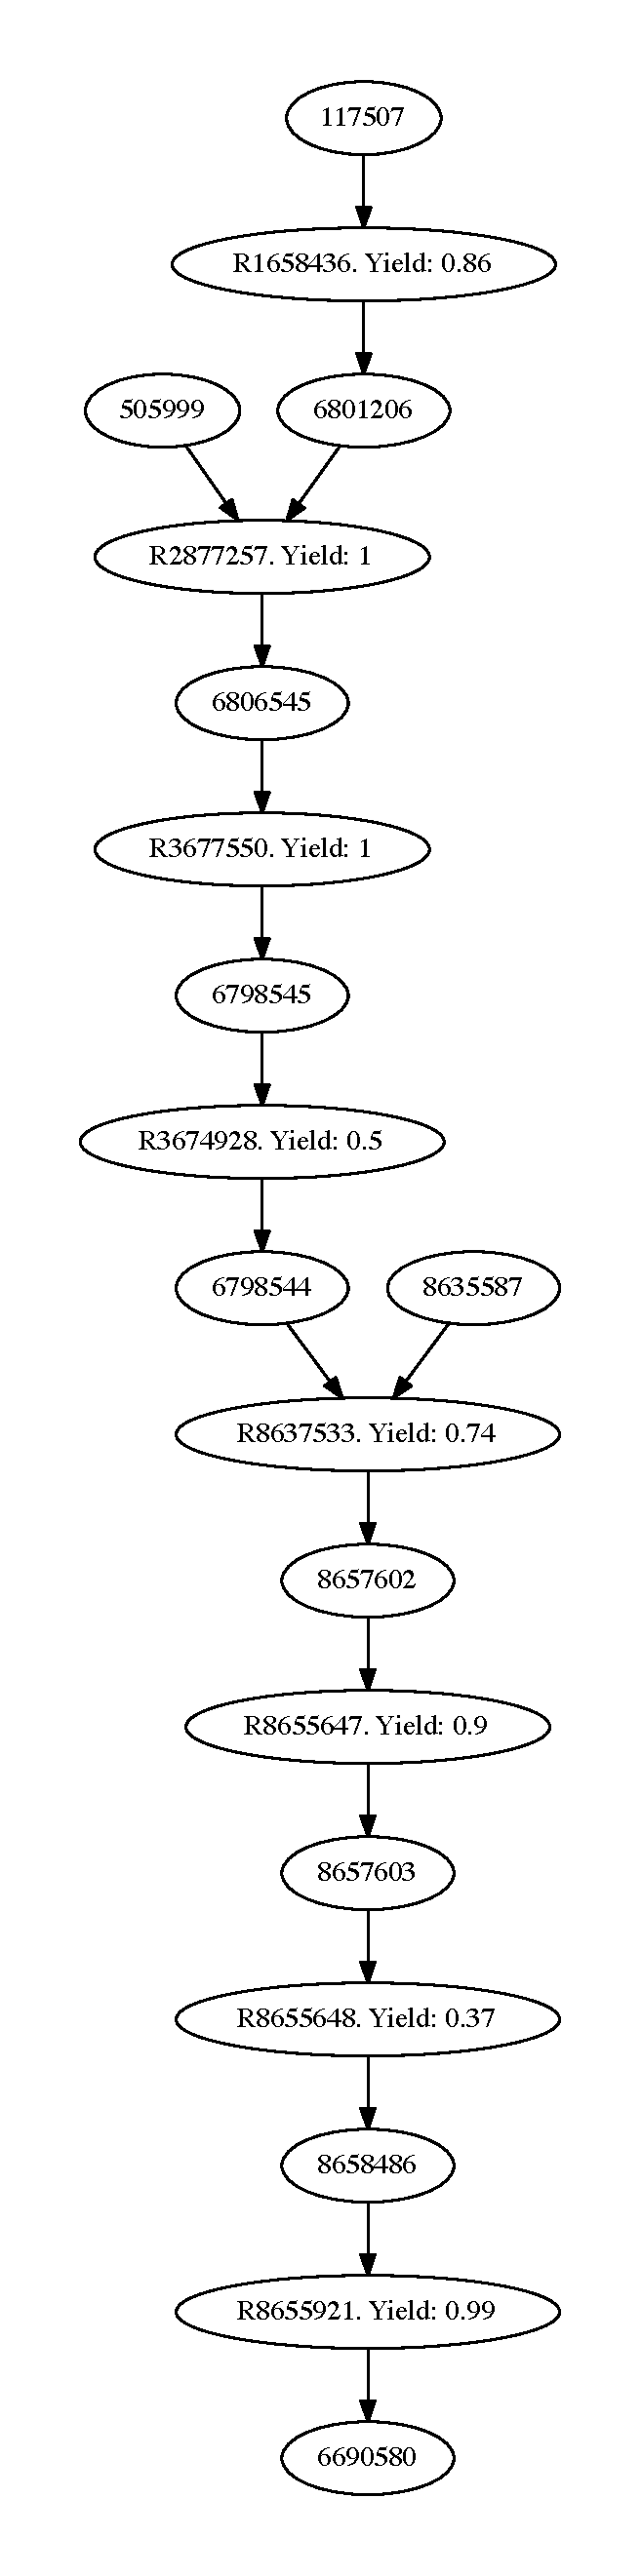
\includegraphics[scale=0.4]{Synteseplaner/Strychnine/plan2.pdf}
\label{Appendix::Strychnine2}

\subsection{Strychnine plan 3}
\centering
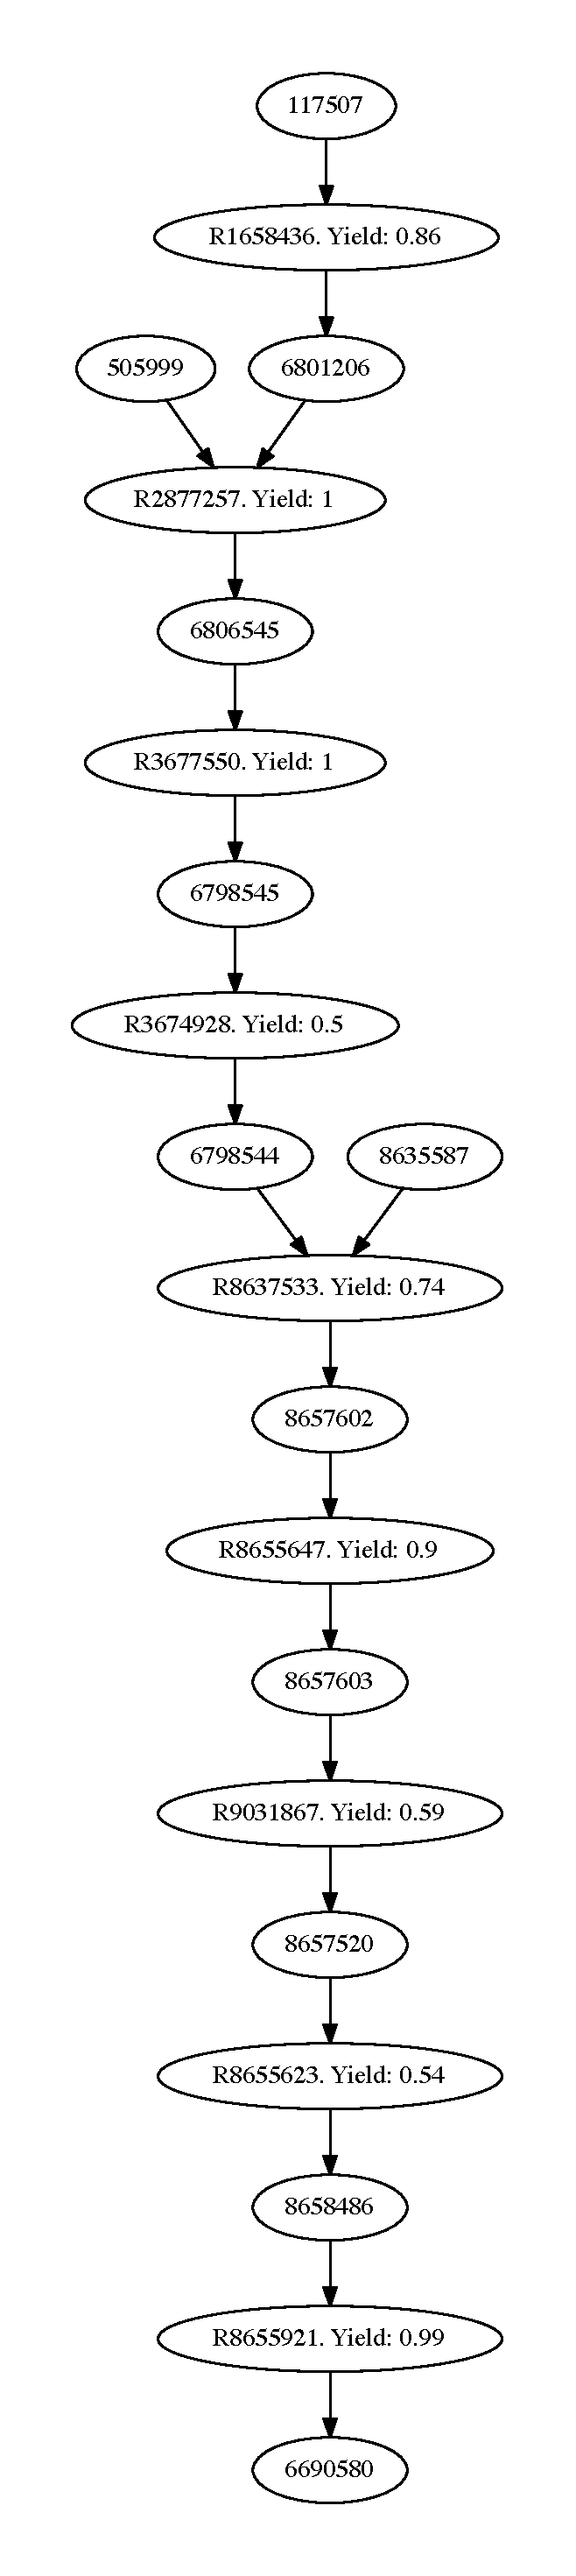
\includegraphics[scale=0.4]{Synteseplaner/Strychnine/plan3.pdf}
\label{Appendix::Strychnine3}


\subsection{Strychnine plan 4}
\centering
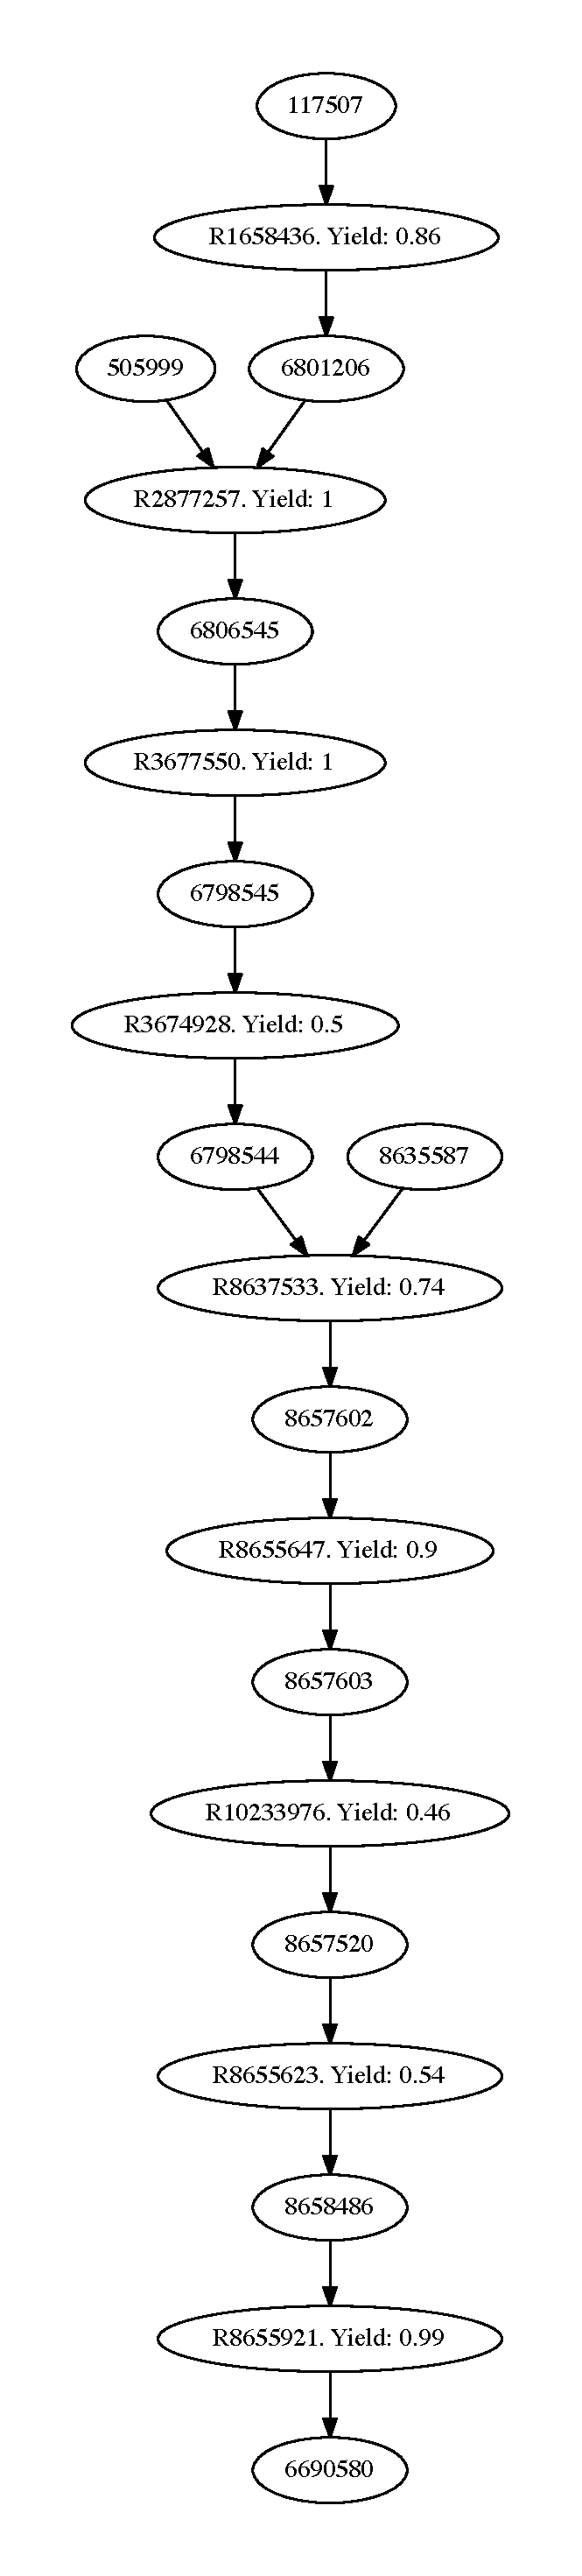
\includegraphics[scale=0.4]{Synteseplaner/Strychnine/plan4.pdf}
\label{Appendix::Strychnine4}

\subsection{Strychnine plan 5}
\centering
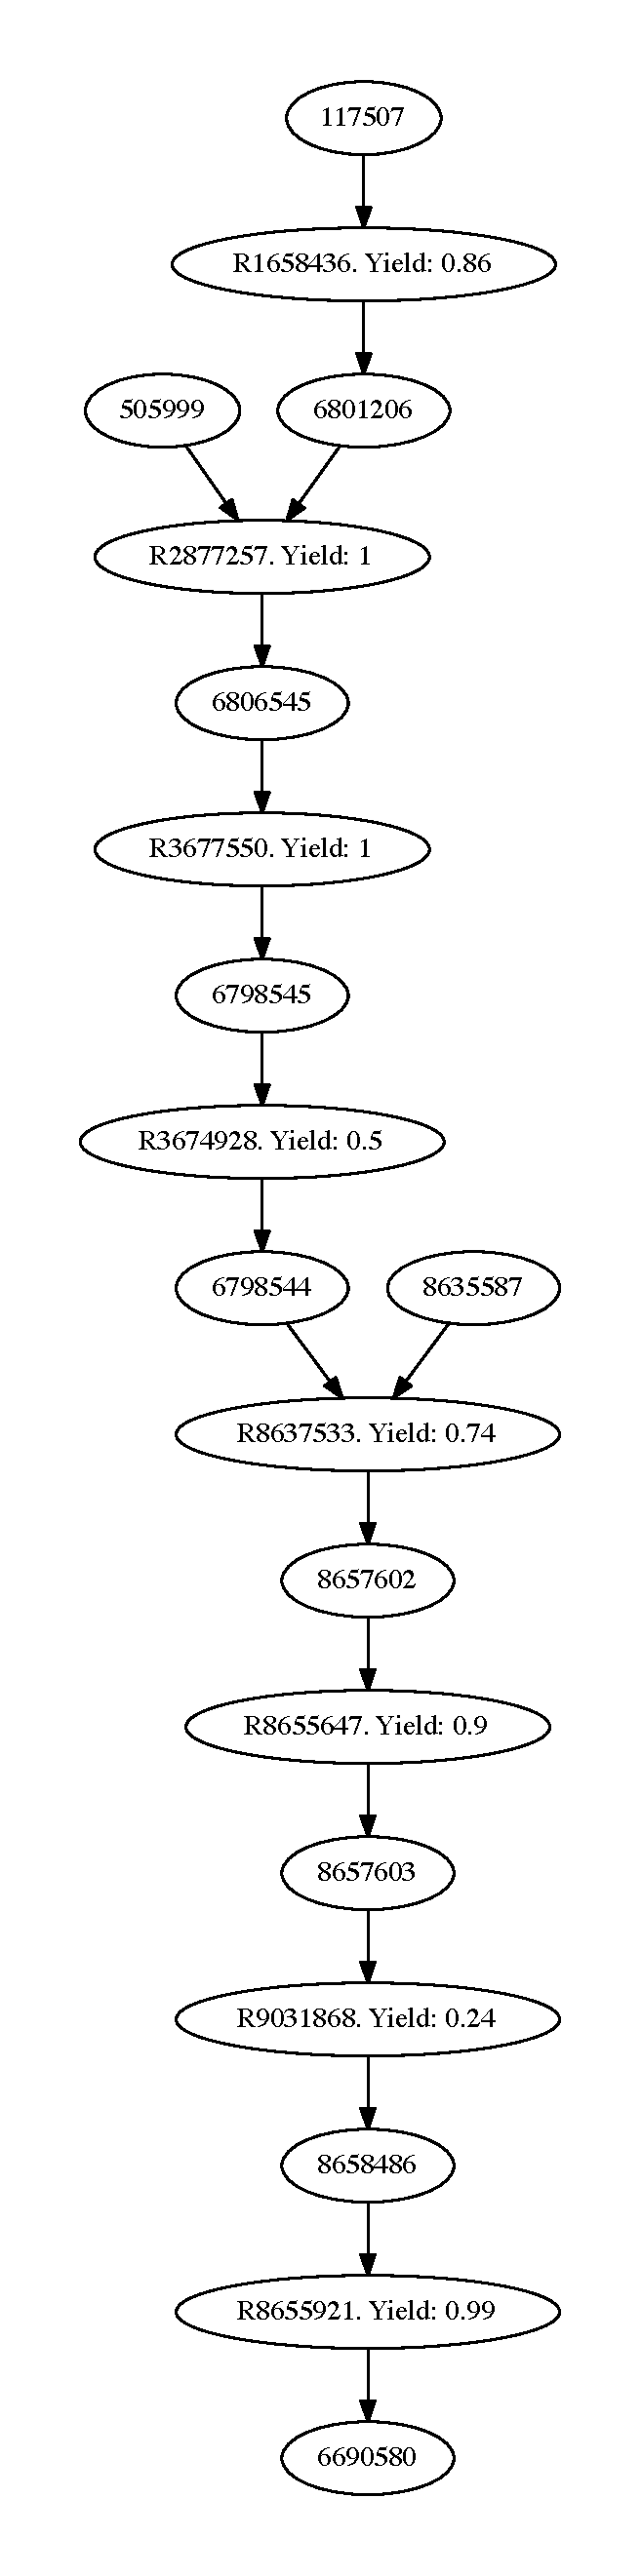
\includegraphics[scale=0.4]{Synteseplaner/Strychnine/plan5.pdf}
\label{Appendix::Strychnine5}


\subsection{Strychnine plan 6}
\centering
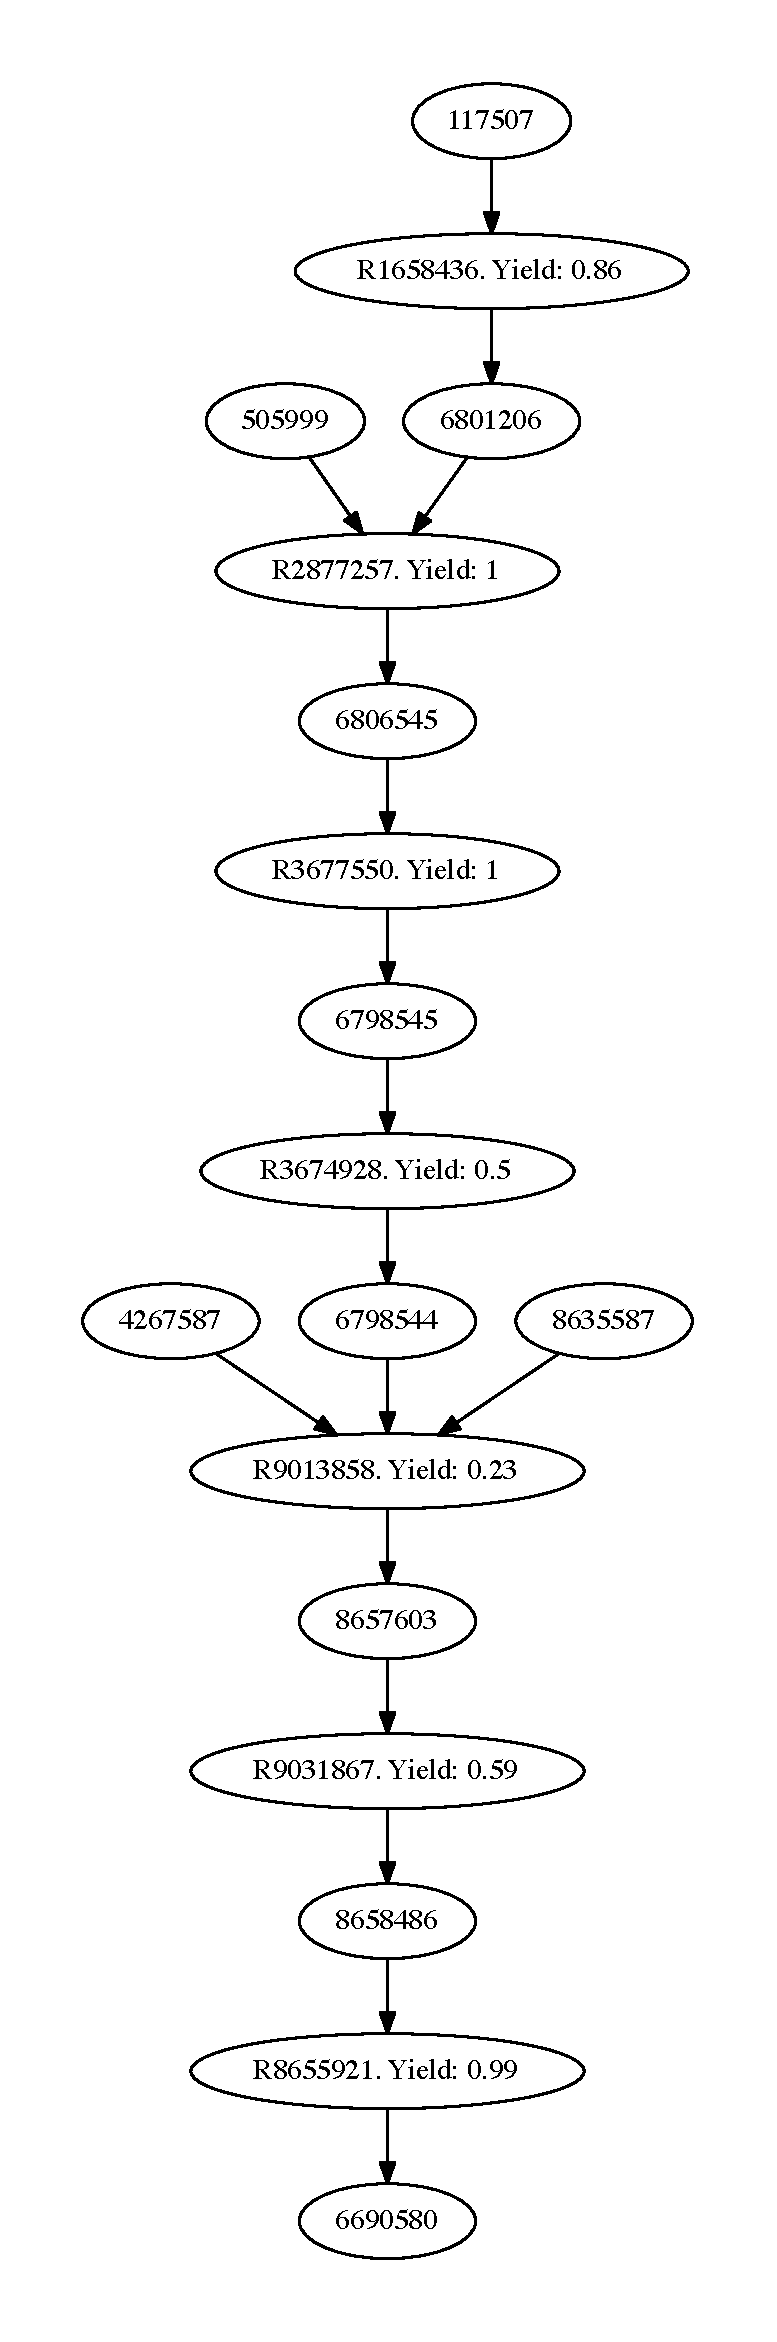
\includegraphics[scale=0.4]{Synteseplaner/Strychnine/plan6.pdf}
\label{Appendix::Strychnine6}

\subsection{Strychnine plan 7}
\centering
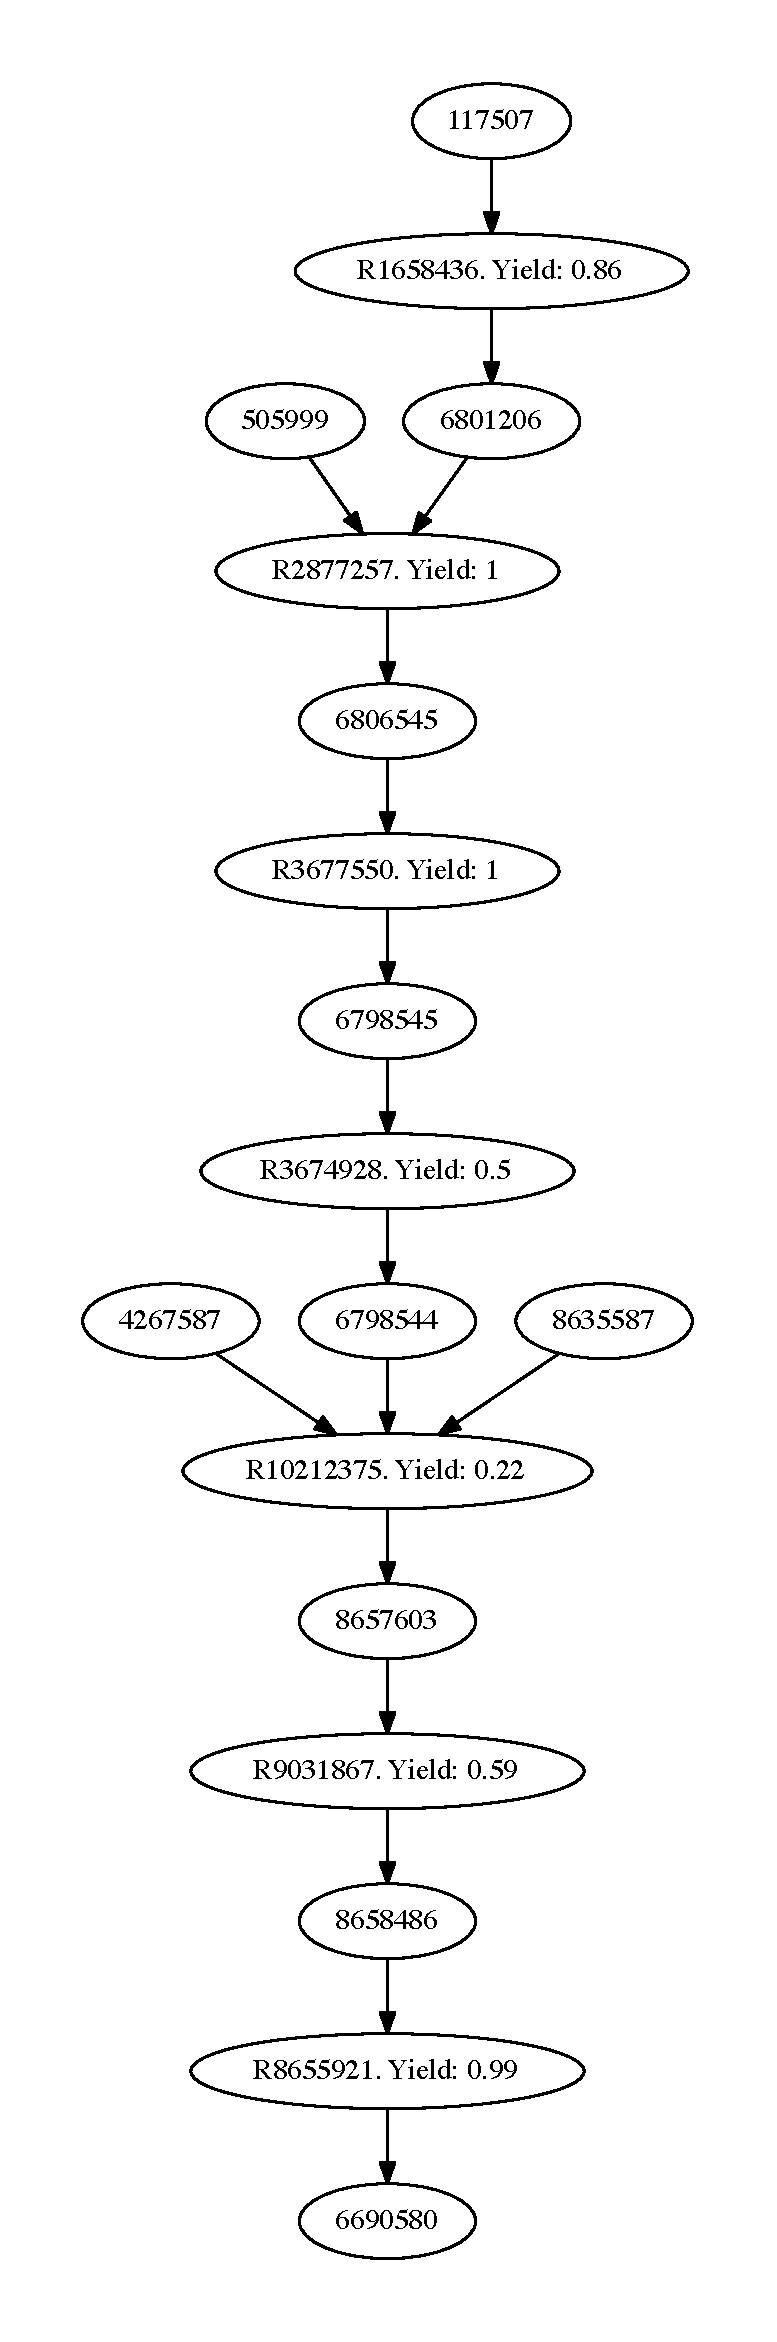
\includegraphics[scale=0.4]{Synteseplaner/Strychnine/plan7.pdf}
\label{Appendix::Strychnine7}


\subsection{Strychnine plan 8}
\centering
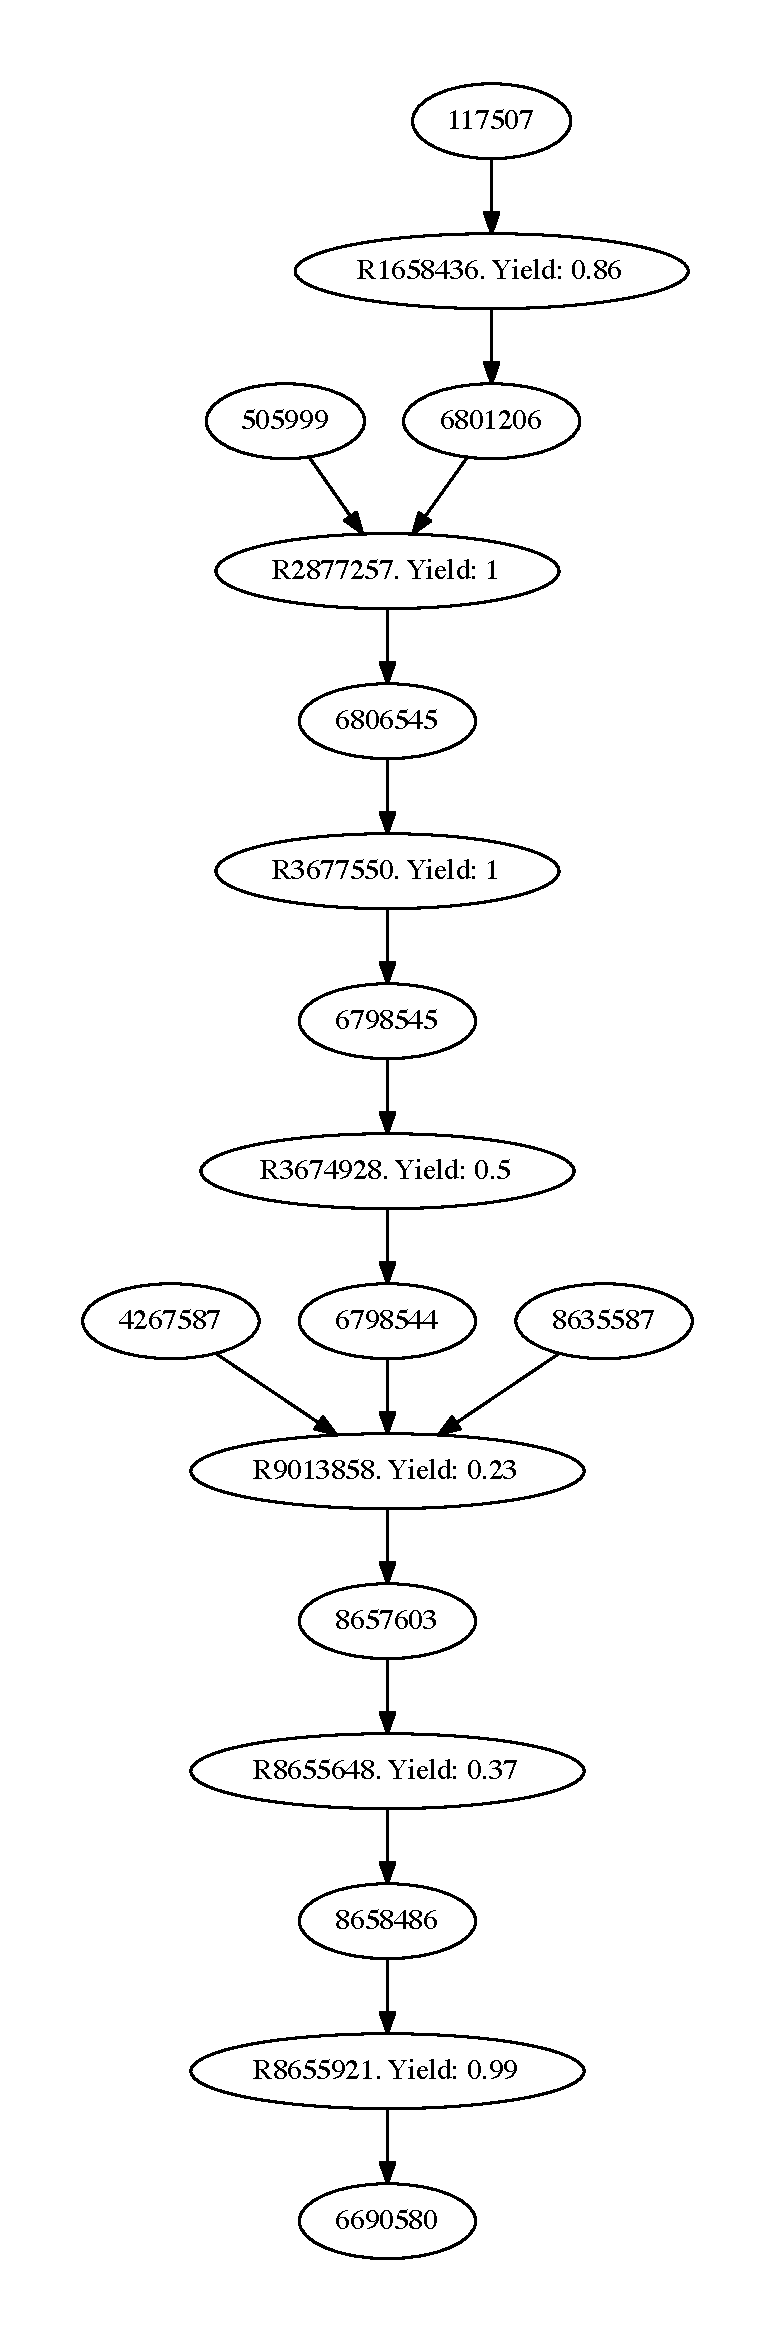
\includegraphics[scale=0.4]{Synteseplaner/Strychnine/plan8.pdf}
\label{Appendix::Strychnine8}

\subsection{Strychnine plan 9}
\centering
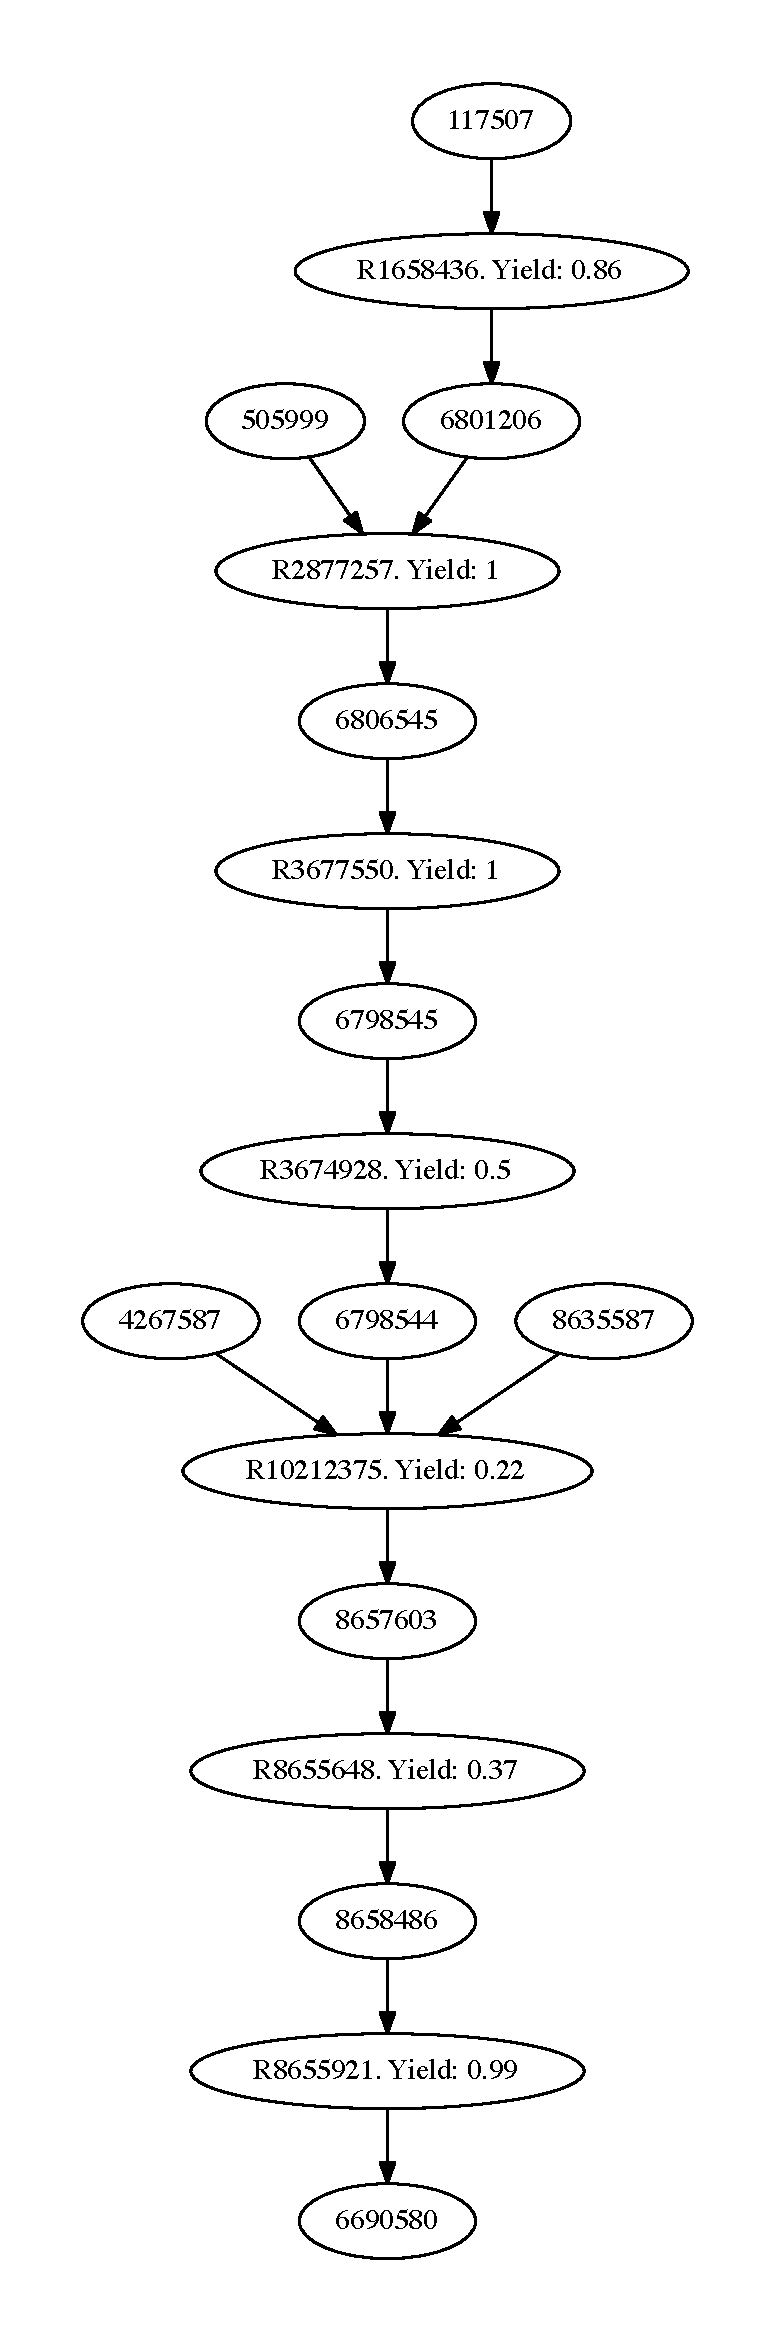
\includegraphics[scale=0.4]{Synteseplaner/Strychnine/plan9.pdf}
\label{Appendix::Strychnine9}

\subsection{Strychnine plan 10}
\centering
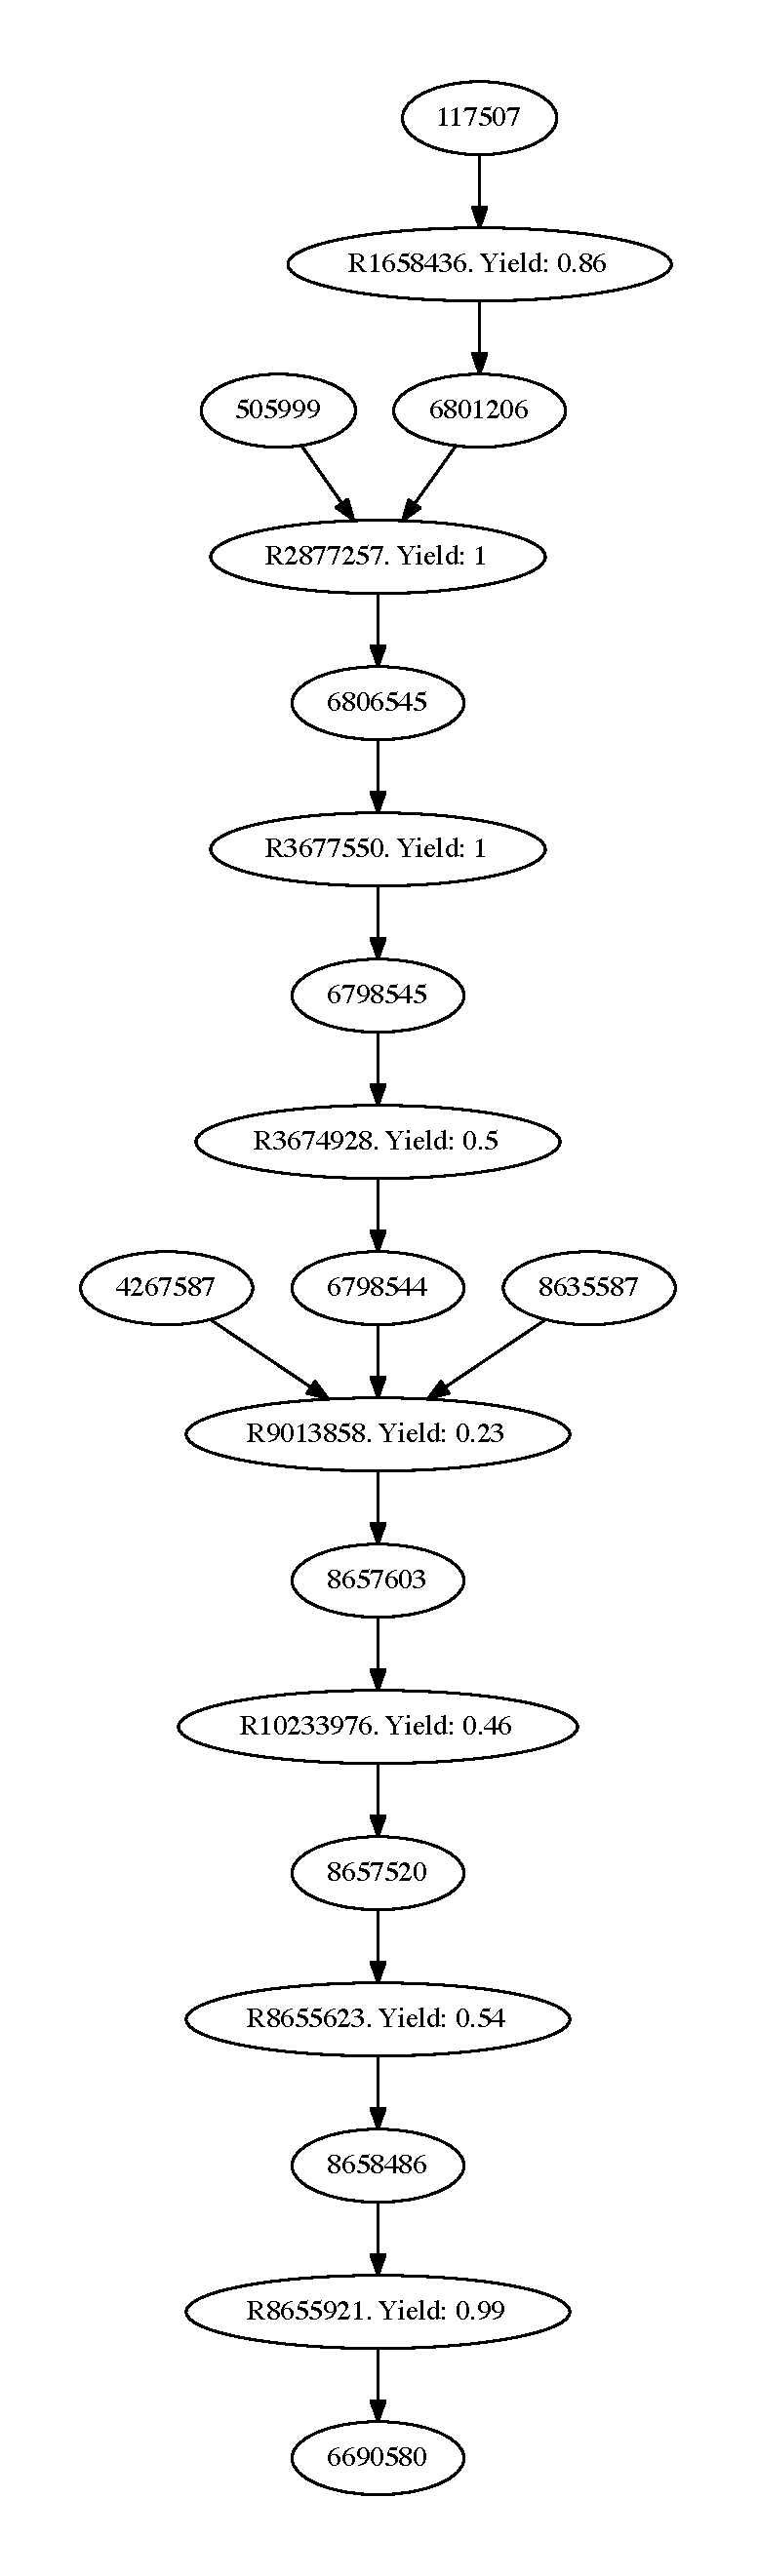
\includegraphics[scale=0.4]{Synteseplaner/Strychnine/plan10.pdf}
\label{Appendix::Strychnine10}

\subsection{Strychnine plan 11}
\centering
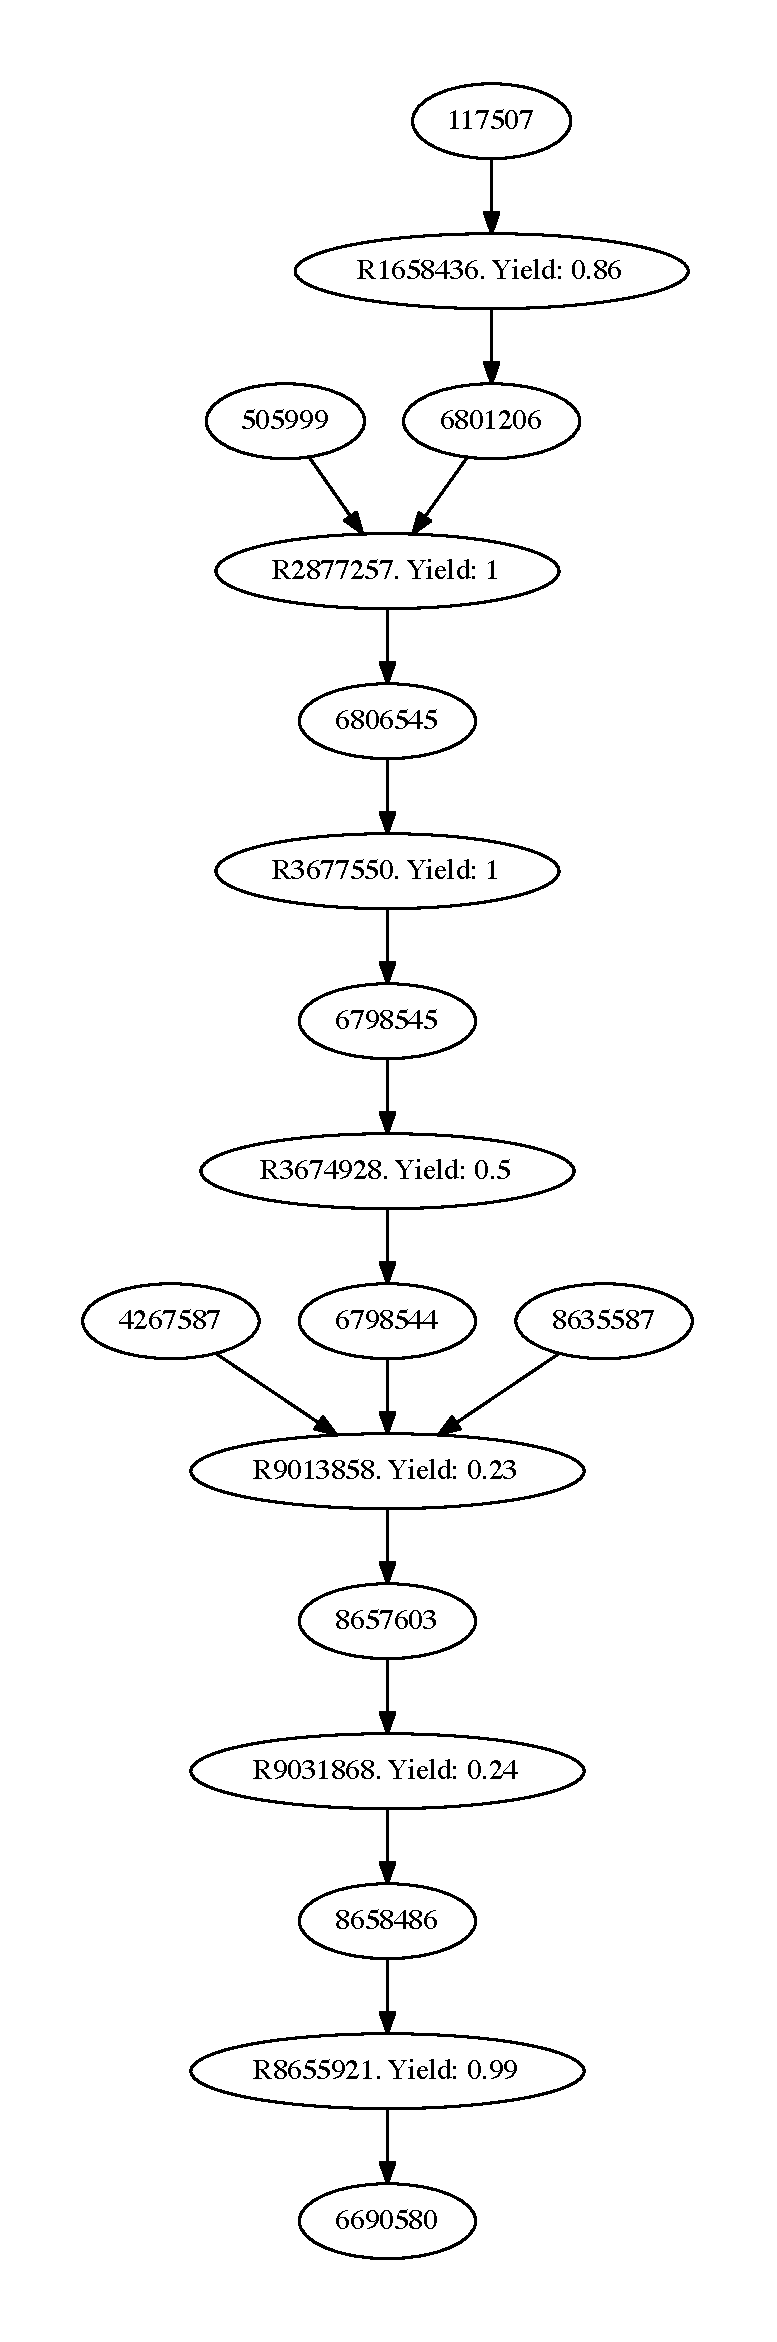
\includegraphics[scale=0.4]{Synteseplaner/Strychnine/plan11.pdf}
\label{Appendix::Strychnine11}

\subsection{Strychnine plan 12}
\centering
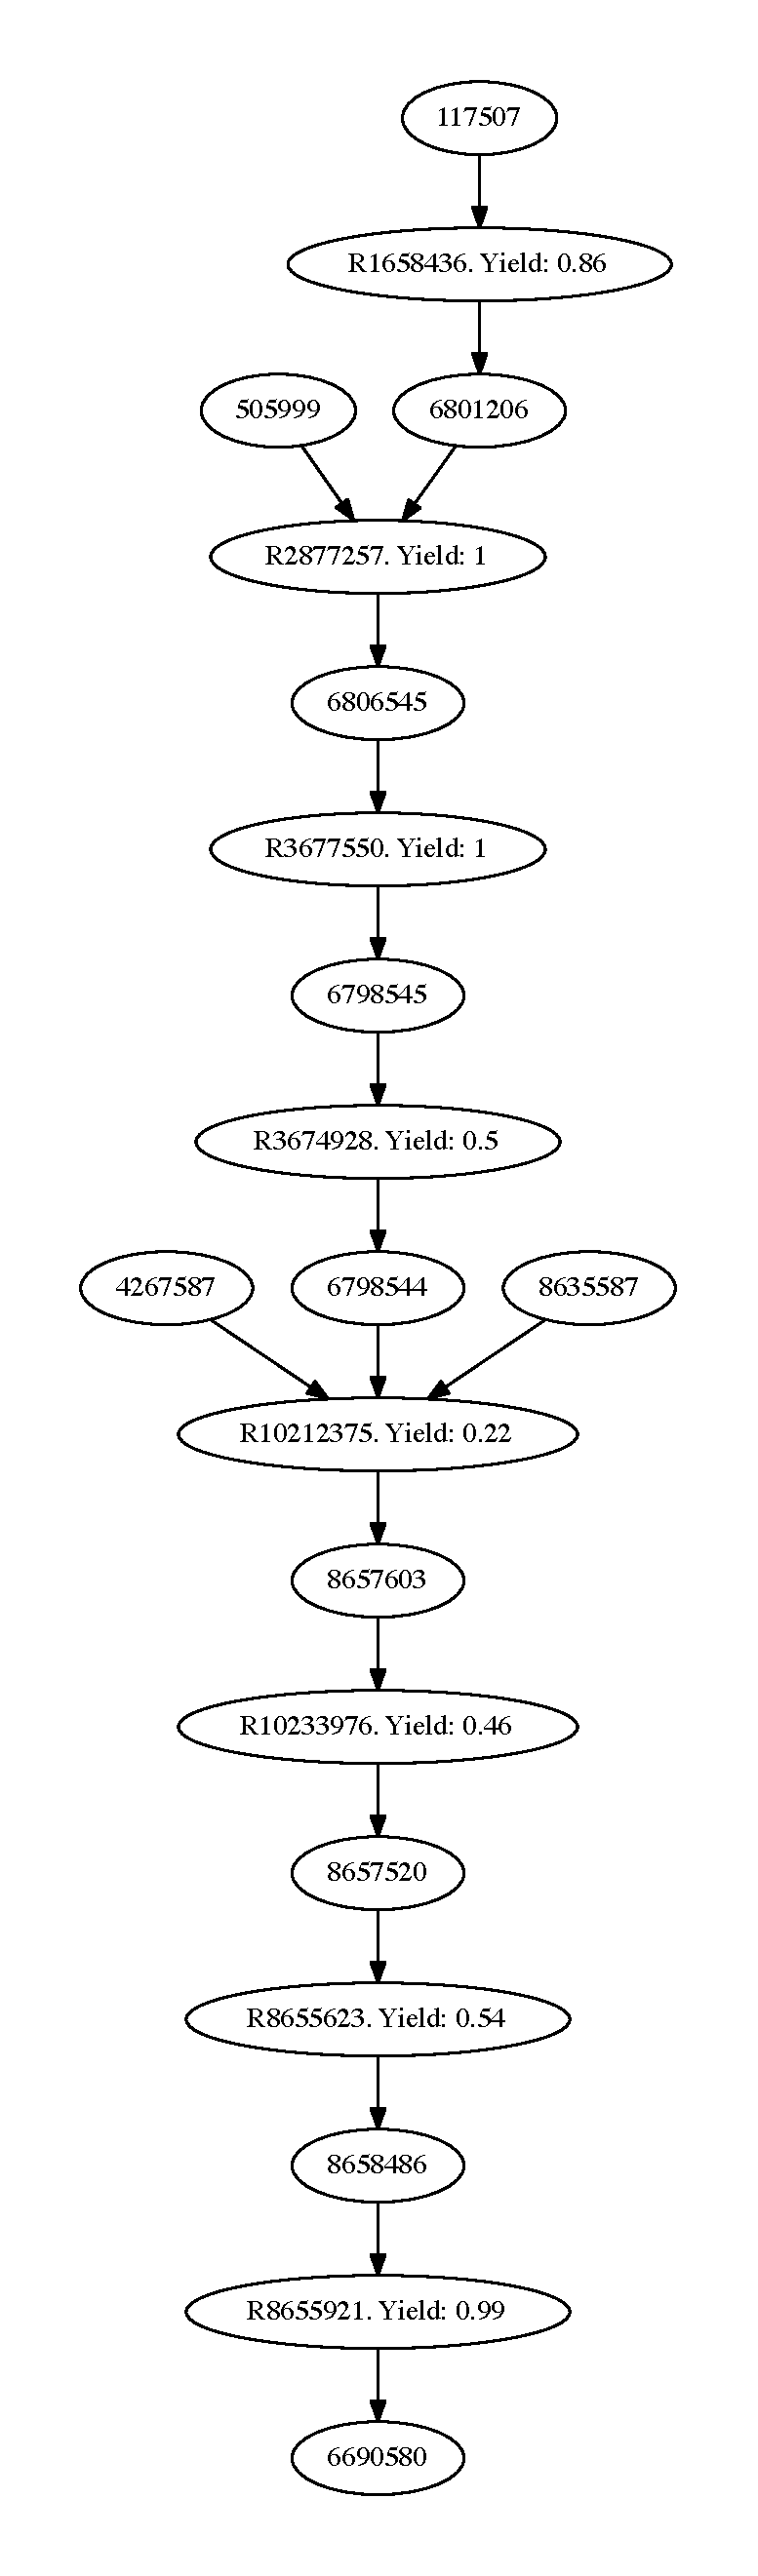
\includegraphics[scale=0.4]{Synteseplaner/Strychnine/plan12.pdf}
\label{Appendix::Strychnine12}

\subsection{Strychnine plan 13}
\centering
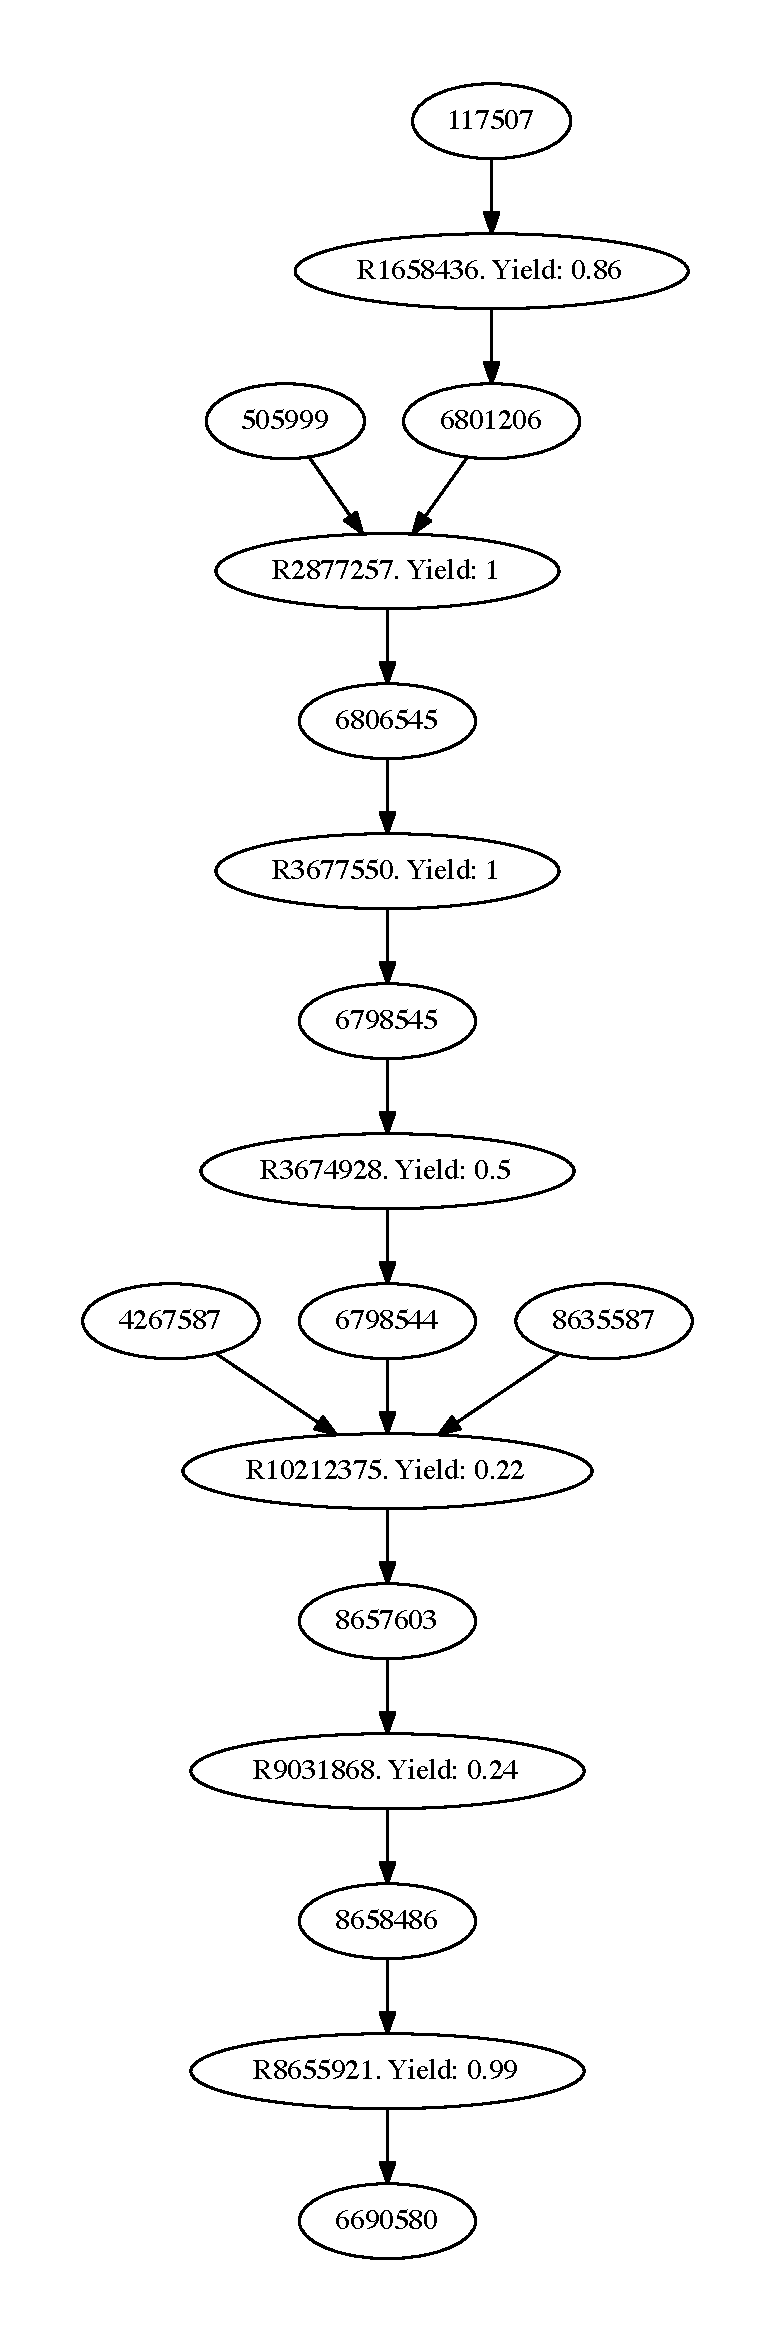
\includegraphics[scale=0.4]{Synteseplaner/Strychnine/plan13.pdf}
\label{Appendix::Strychnine13}

\subsection{Strychnine plan 14}
\centering
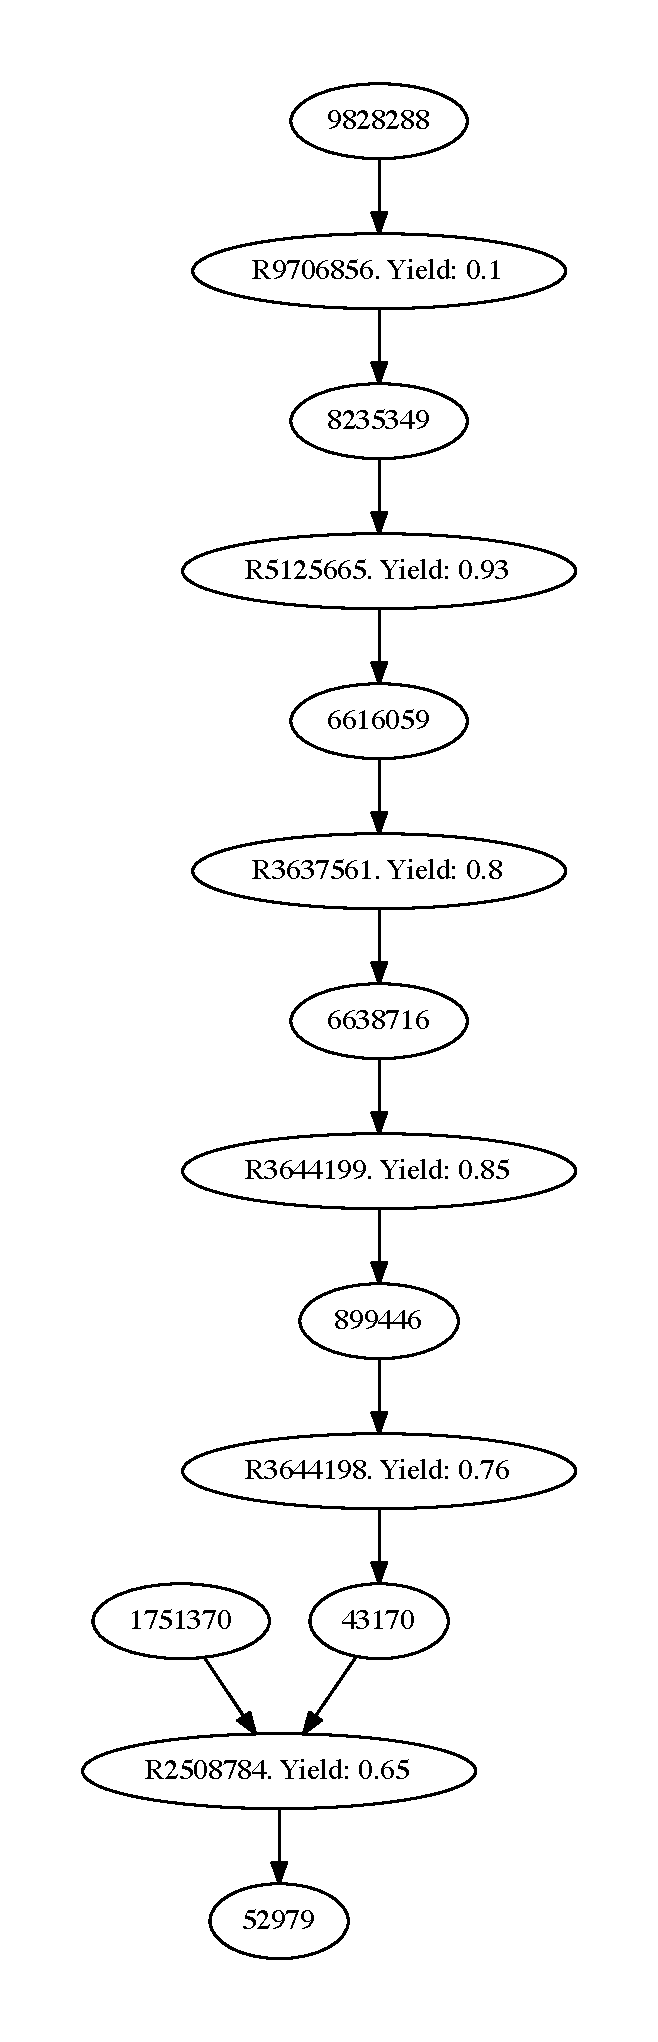
\includegraphics[scale=0.4]{Synteseplaner/Strychnine/plan14.pdf}
\label{Appendix::Strychnine14}

\subsection{Strychnine plan 15}
\centering
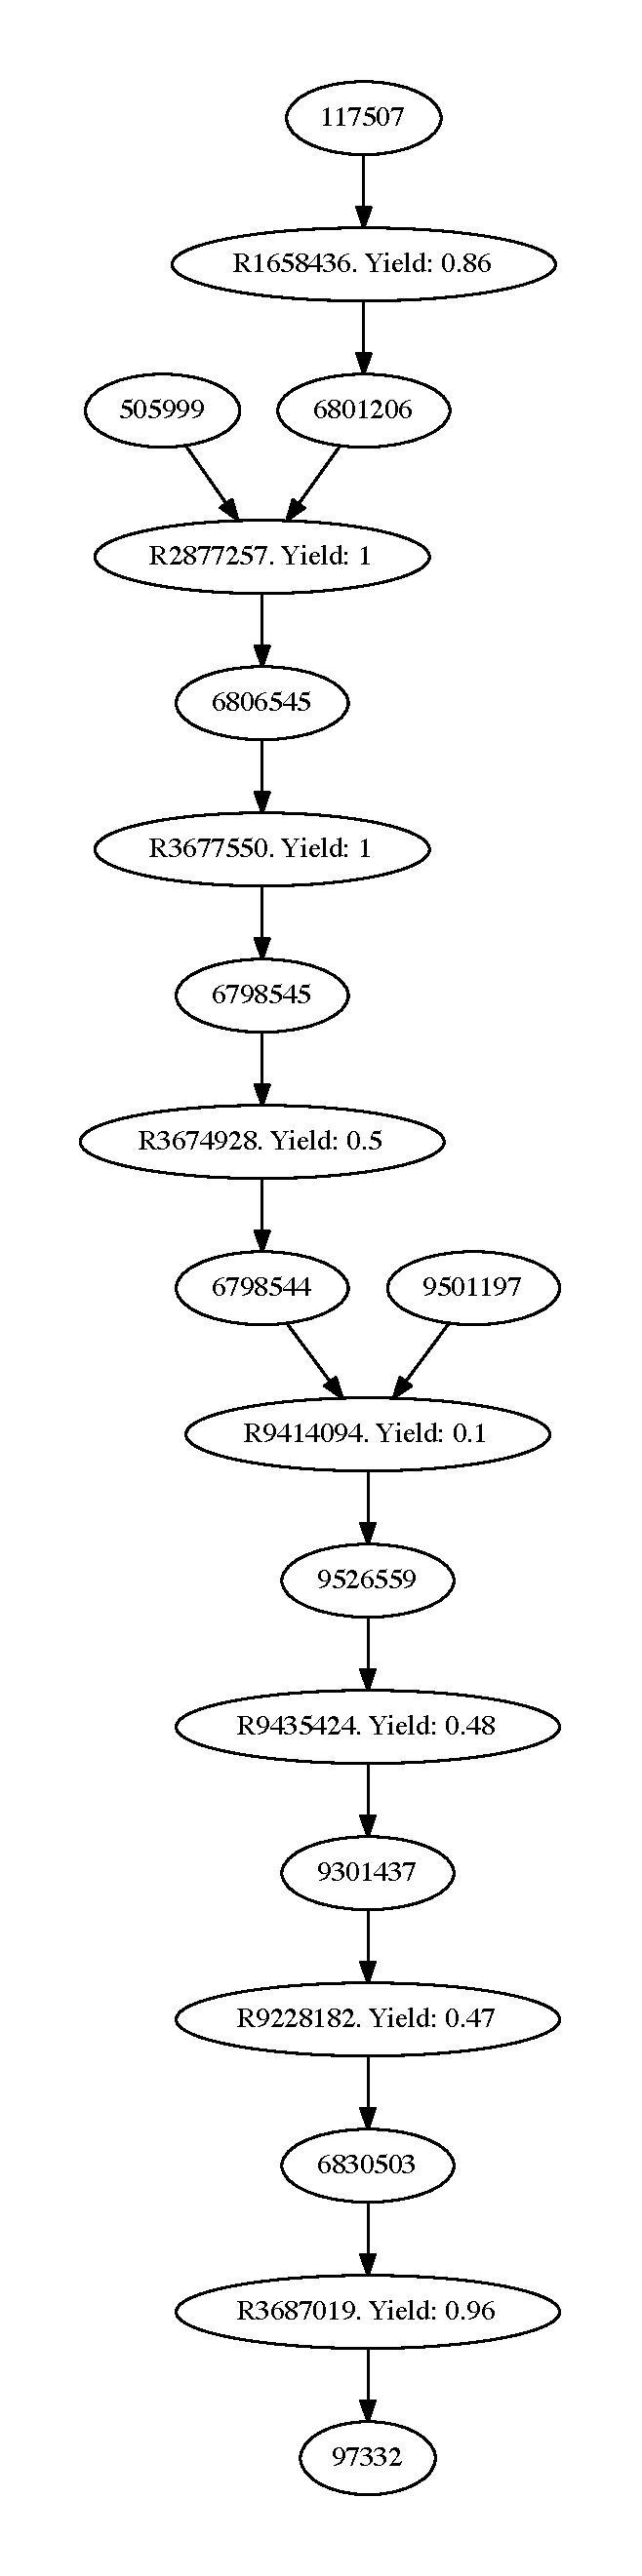
\includegraphics[scale=0.4]{Synteseplaner/Strychnine/plan15.pdf}
\label{Appendix::Strychnine15}

\subsection{Strychnine plan 16}
\centering
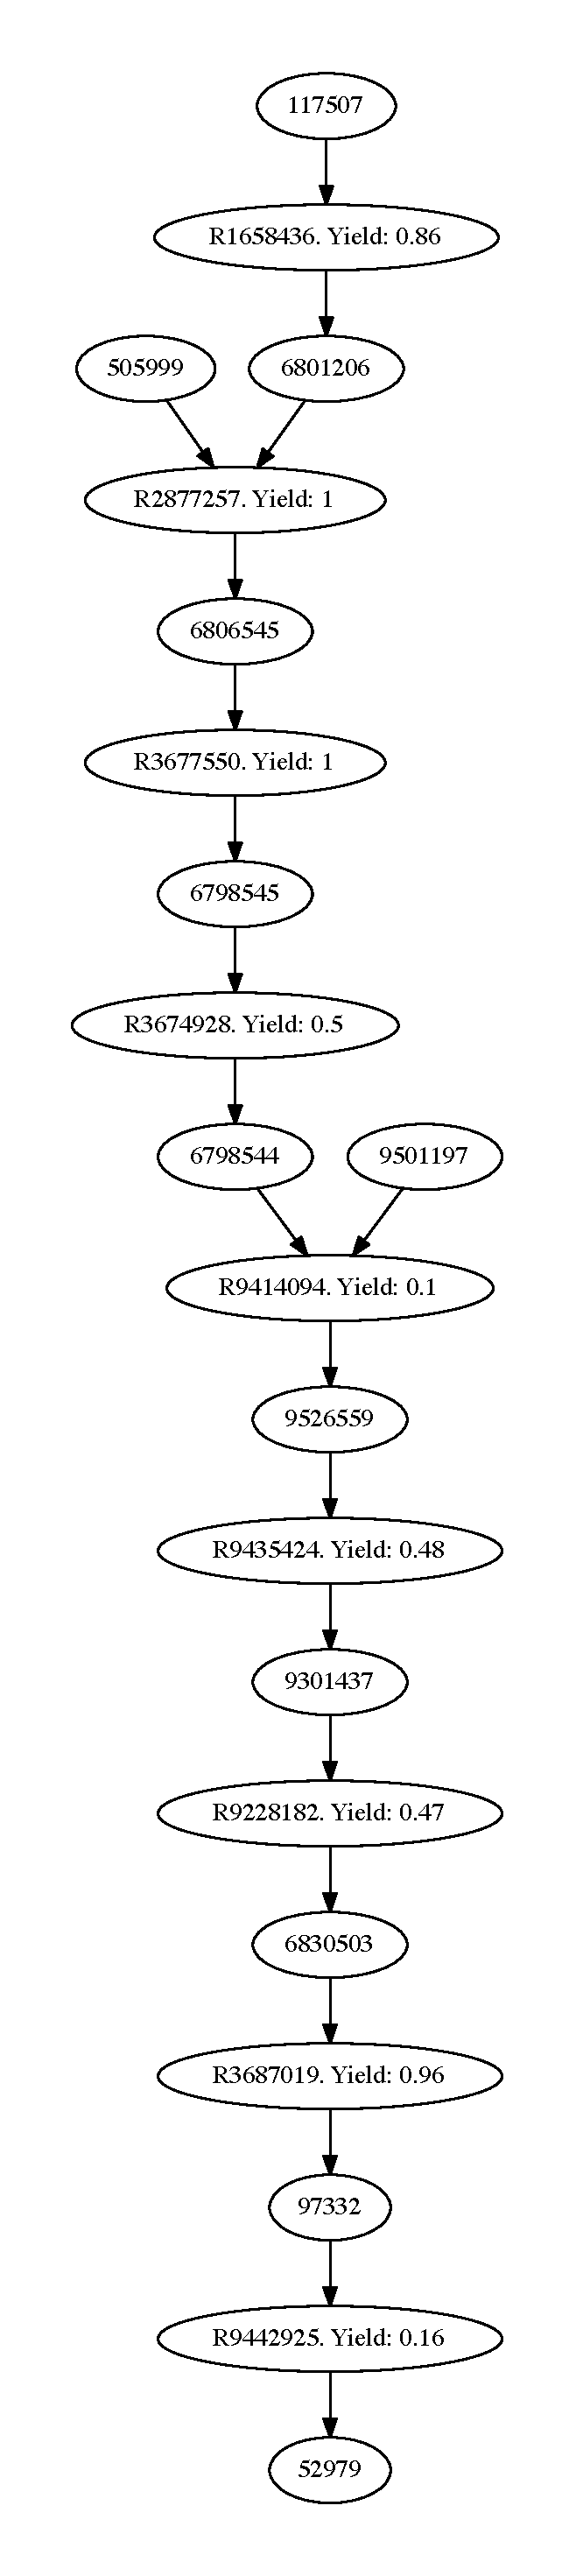
\includegraphics[scale=0.4]{Synteseplaner/Strychnine/plan16.pdf}
\label{Appendix::Strychnine16}

\subsection{Colchicine plan 1}
\centering
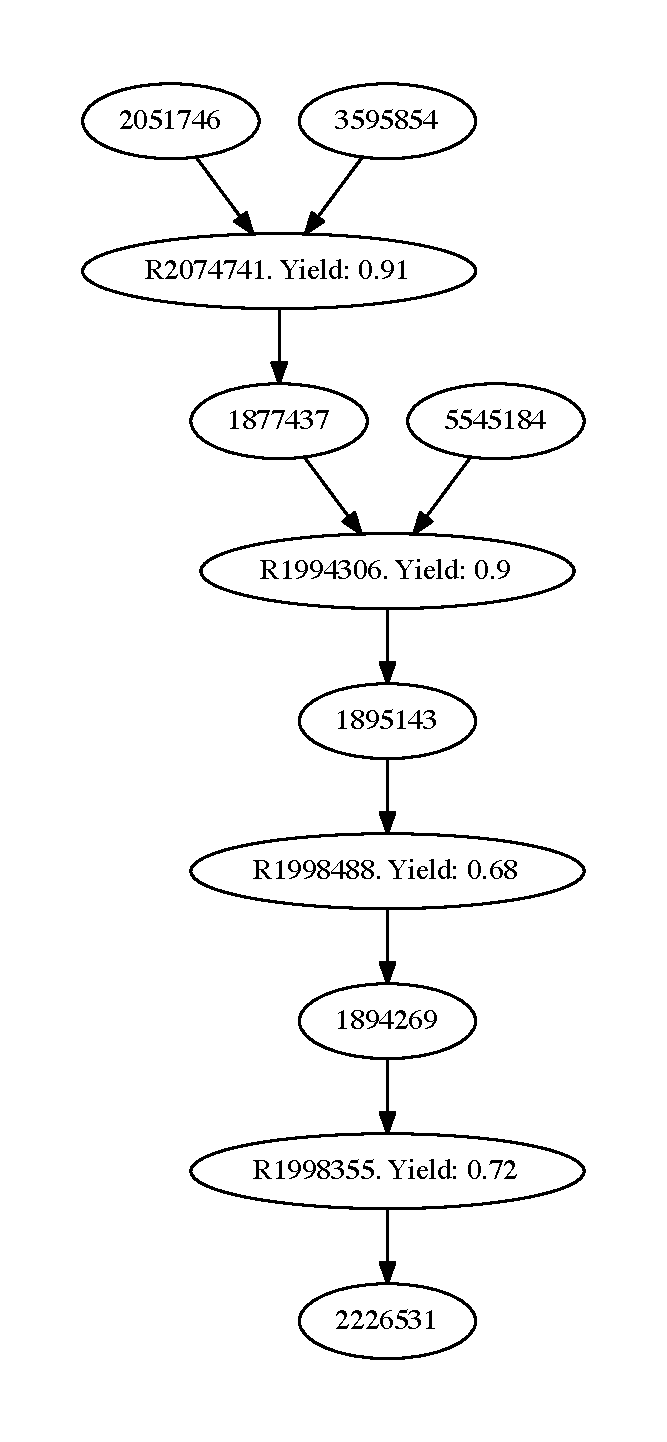
\includegraphics[scale=0.4]{Synteseplaner/Colchicine/plan1.pdf}
\label{Appendix::Colchicine1}

\subsection{Colchicine plan 2}
\centering
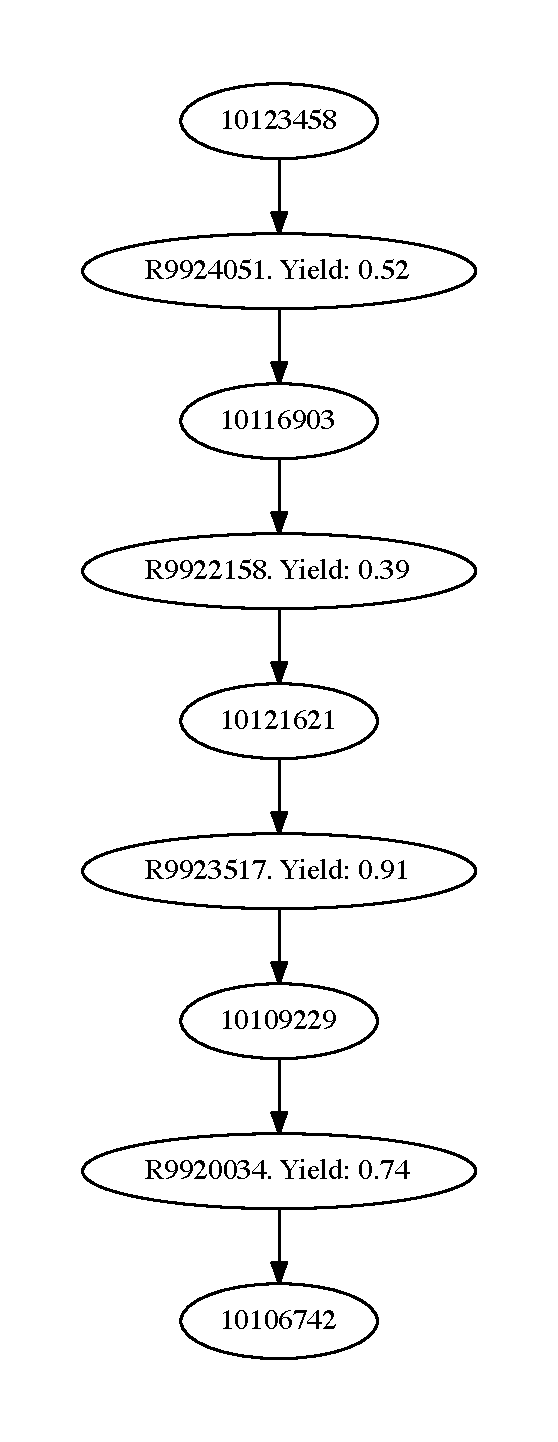
\includegraphics[scale=0.4]{Synteseplaner/Colchicine/plan2.pdf}
\label{Appendix::Colchicine2}

\subsection{Colchicine plan 3}
\centering
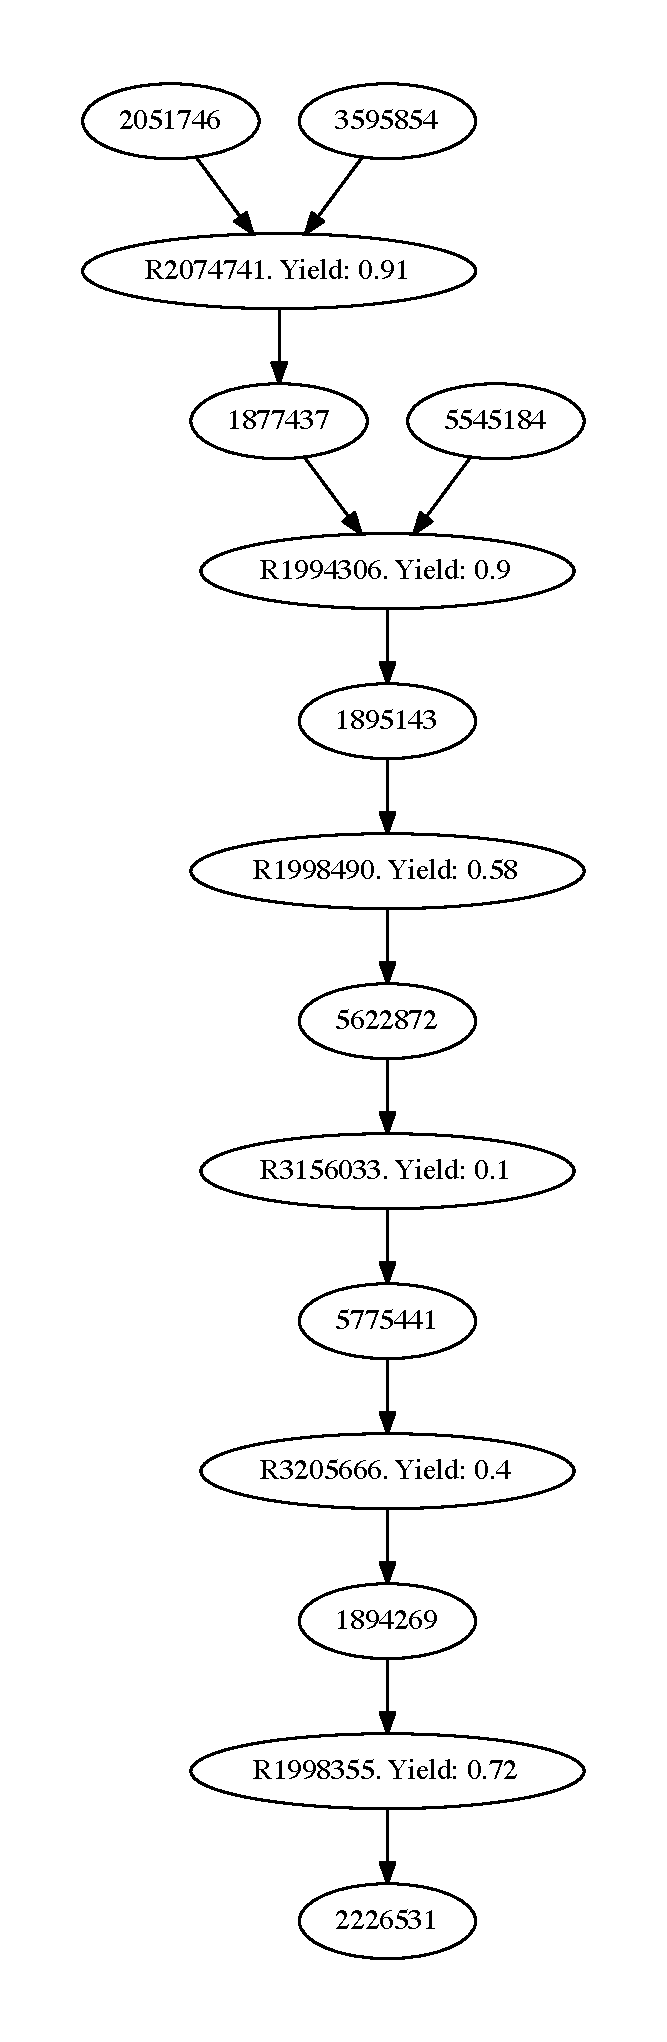
\includegraphics[scale=0.4]{Synteseplaner/Colchicine/plan3.pdf}
\label{Appendix::Colchicine3}

\subsection{Colchicine plan 4}
\centering
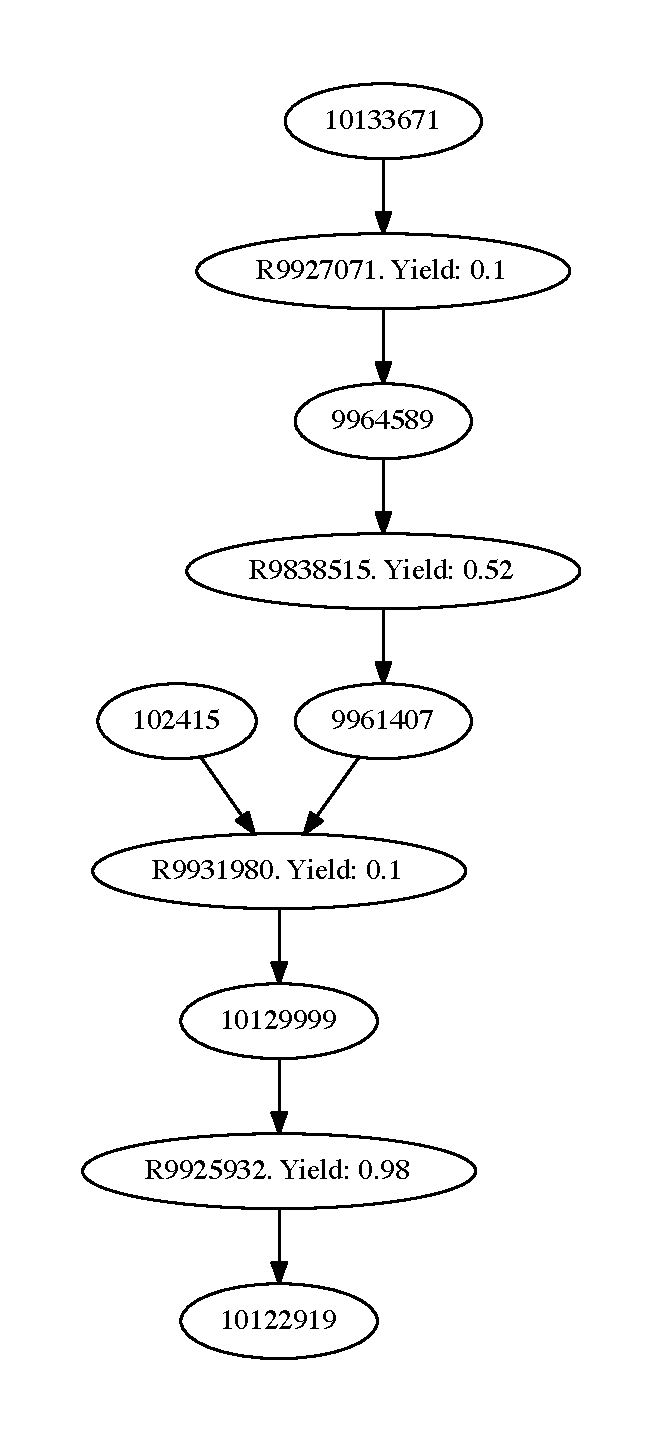
\includegraphics[scale=0.4]{Synteseplaner/Colchicine/plan4.pdf}
\label{Appendix::Colchicine4}

\subsection{Colchicine plan 5}
\centering
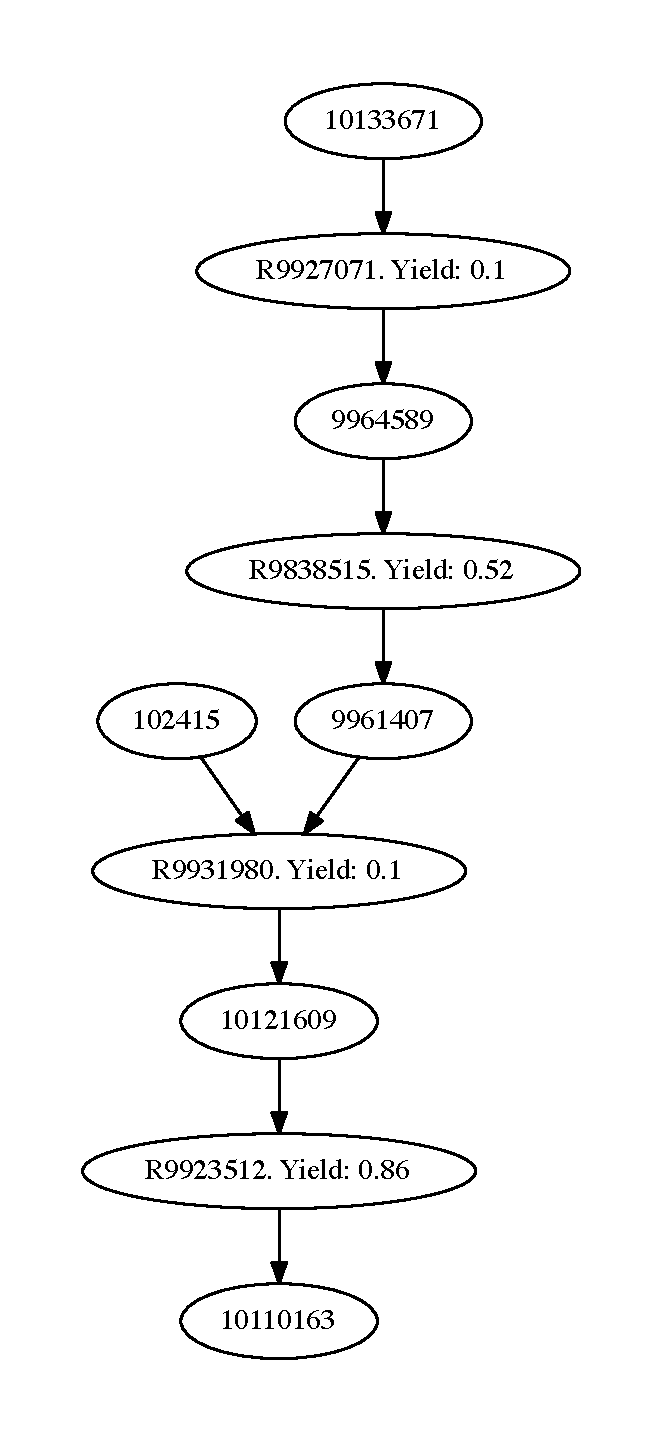
\includegraphics[scale=0.4]{Synteseplaner/Colchicine/plan5.pdf}
\label{Appendix::Colchicine5}

\subsection{Dysidiolide plan 1}
\centering
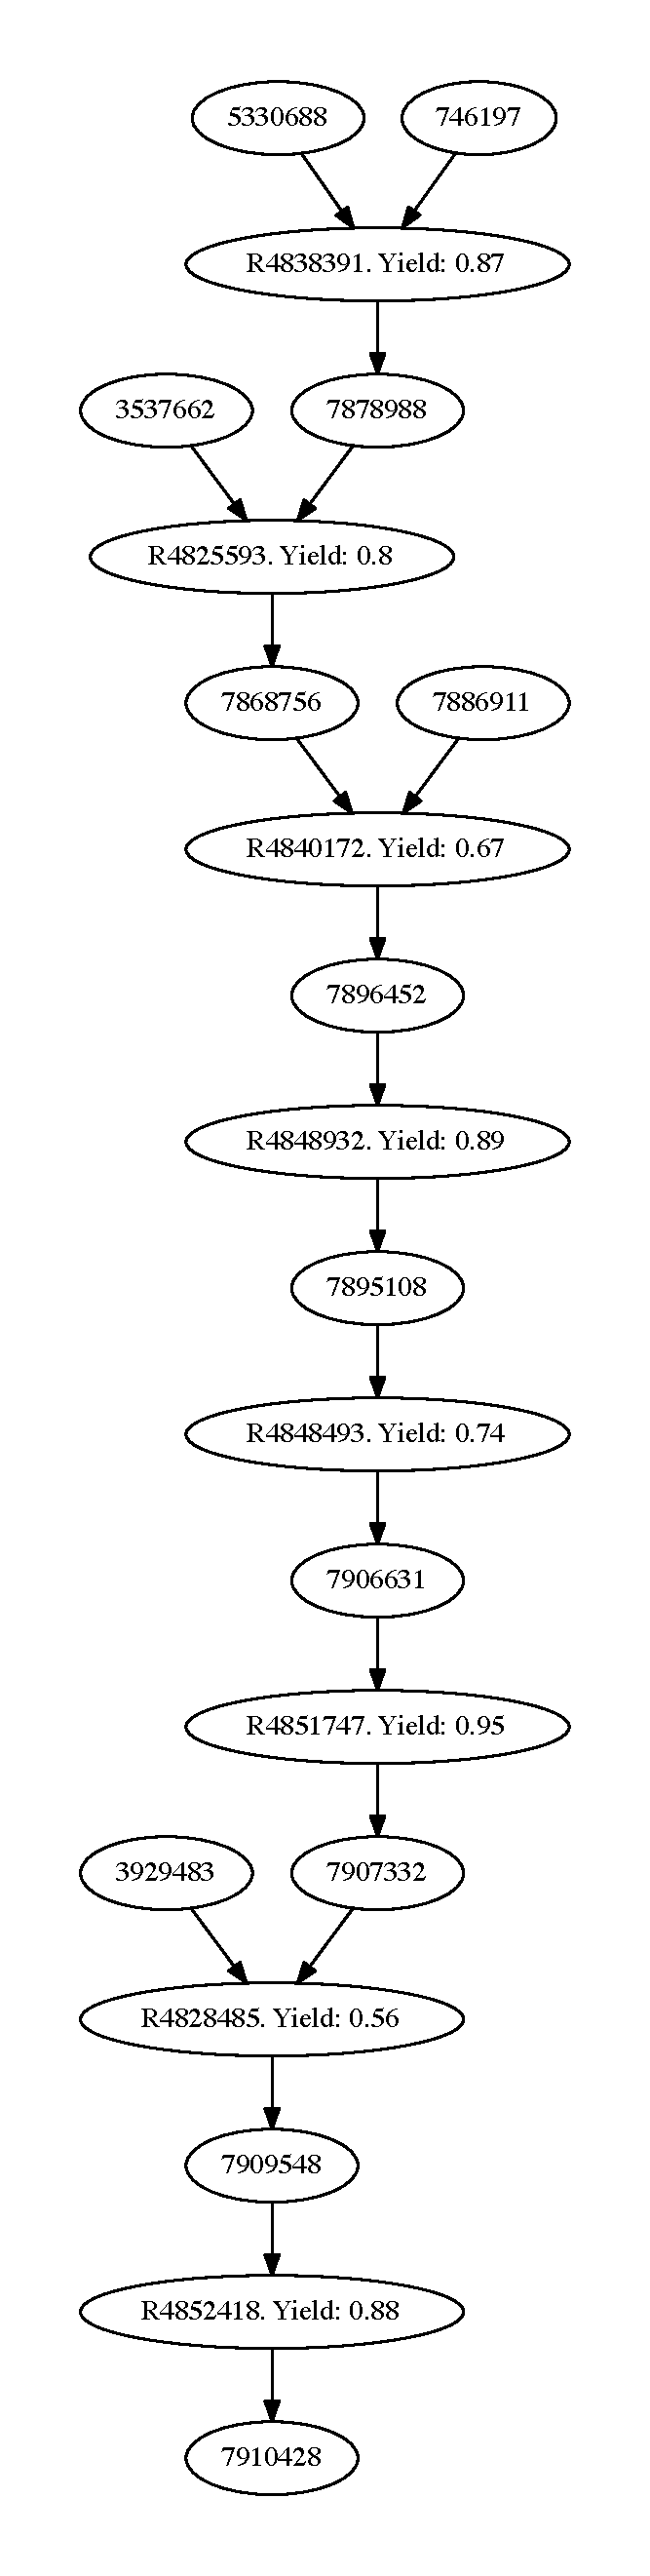
\includegraphics[scale=0.43]{Synteseplaner/Dysidiolide/plan1.pdf}
\label{Appendix::Dysidiolide1}

\subsection{Dysidiolide plan 2}
\centering
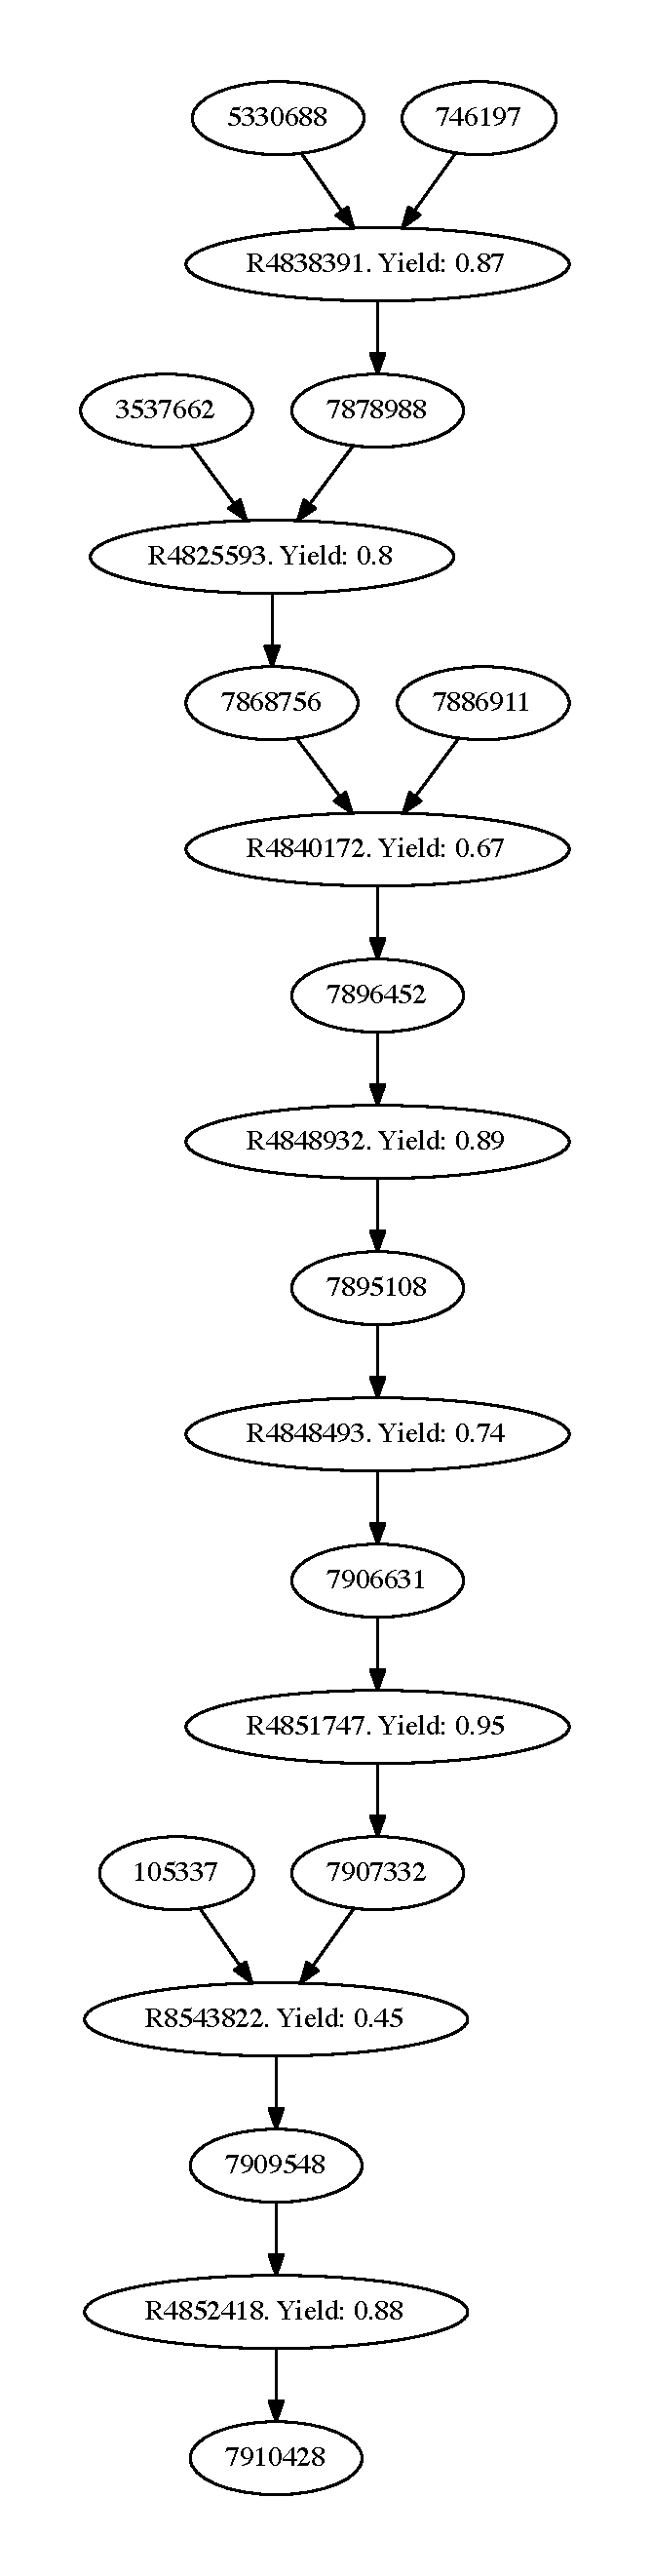
\includegraphics[scale=0.43]{Synteseplaner/Dysidiolide/plan2.pdf}
\label{Appendix::Dysidiolide2}

\subsection{Dysidiolide plan 3}
\centering
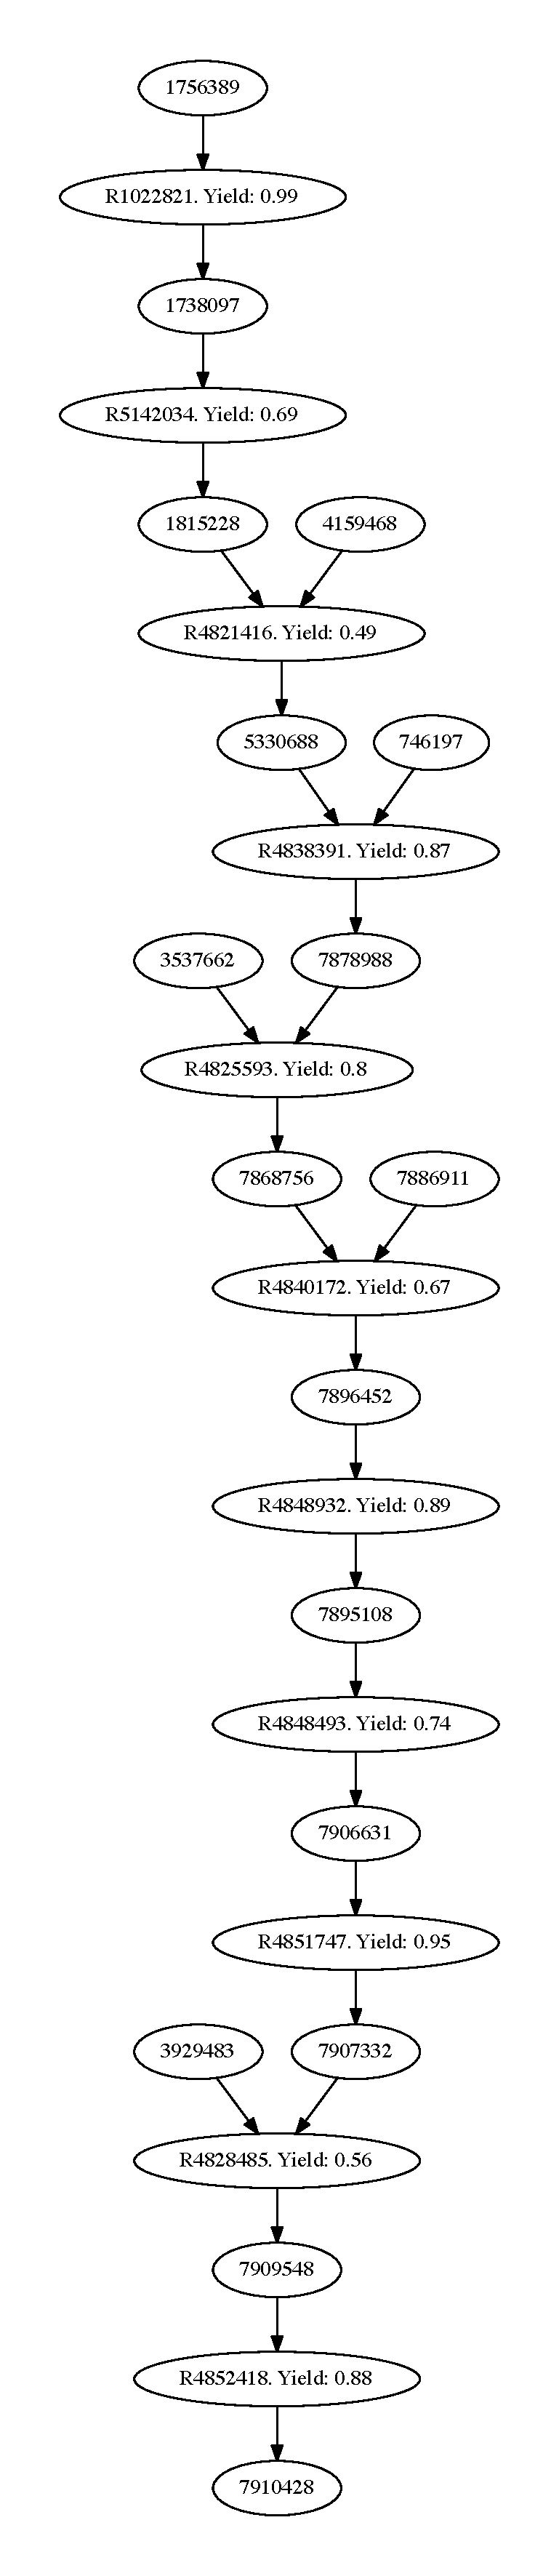
\includegraphics[scale=0.34]{Synteseplaner/Dysidiolide/plan3.pdf}
\label{Appendix::Dysidiolide3}

\subsection{Dysidiolide plan 4}
\centering
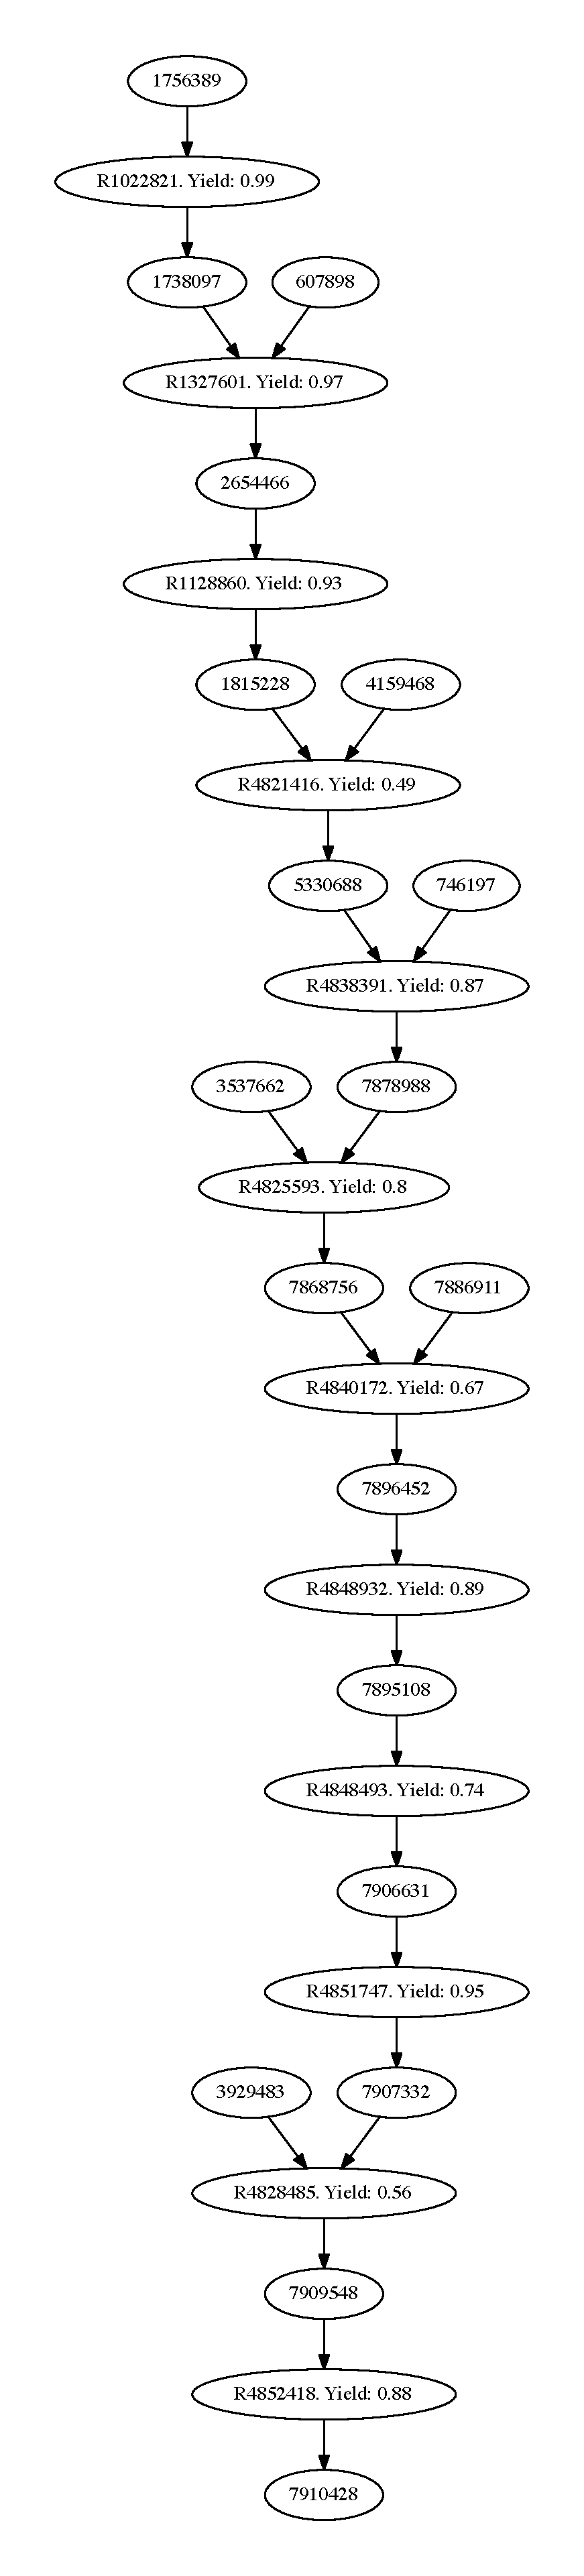
\includegraphics[scale=0.3]{Synteseplaner/Dysidiolide/plan4.pdf}
\label{Appendix::Dysidiolide4}

\subsection{Dysidiolide plan 5}
\centering
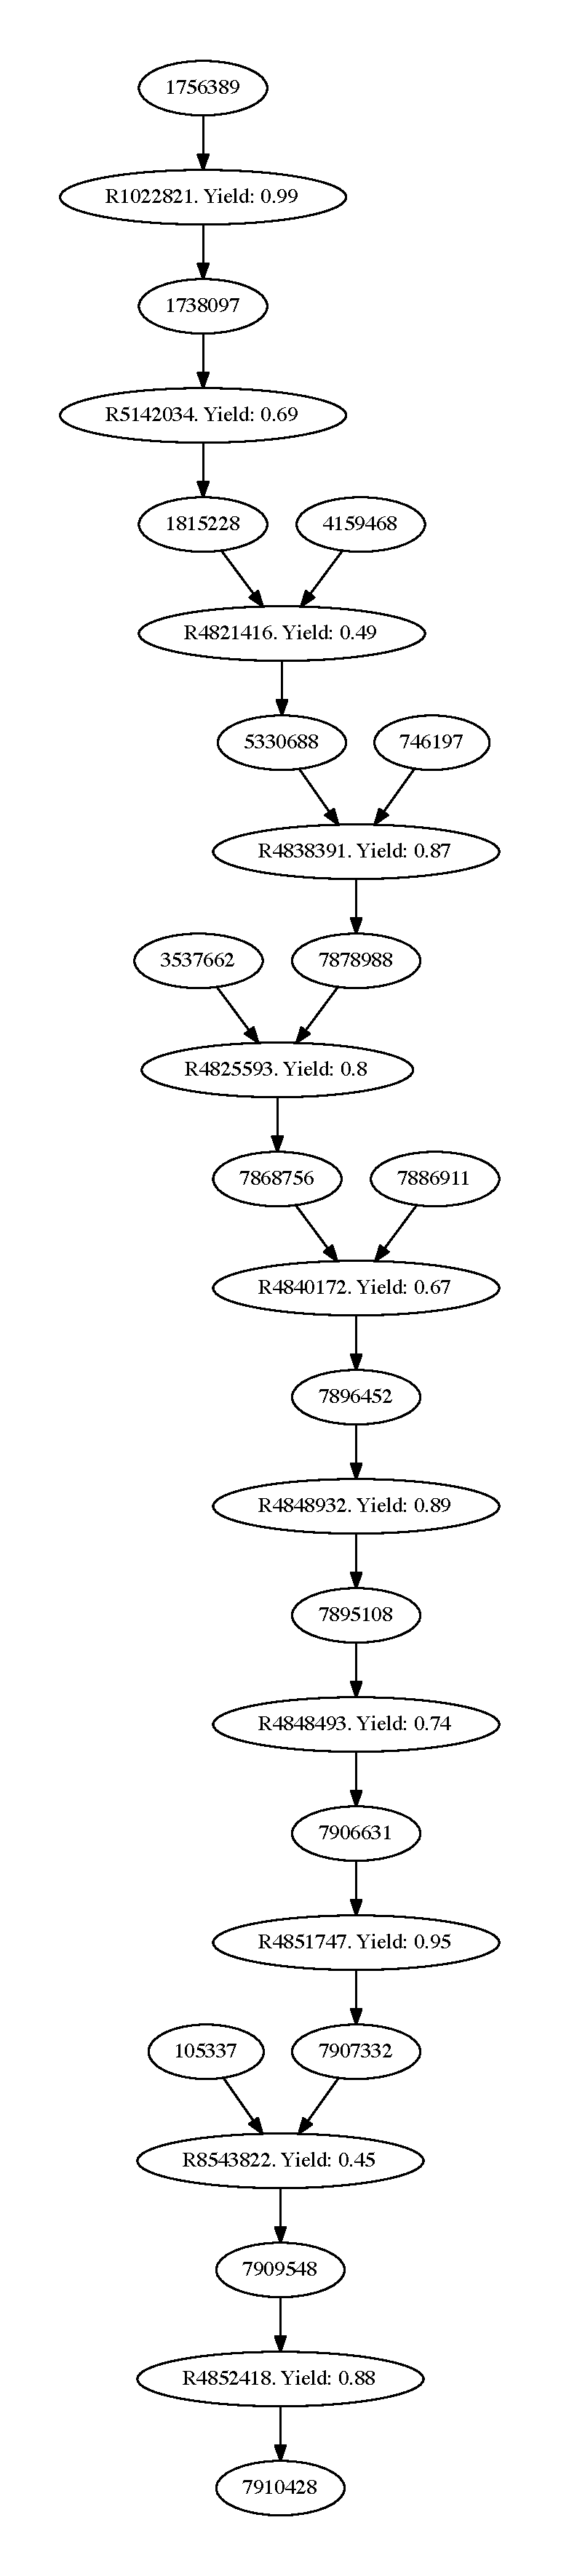
\includegraphics[scale=0.35]{Synteseplaner/Dysidiolide/plan5.pdf}
\label{Appendix::Dysidiolide5}

\subsection{Dysidiolide plan 6}
\centering
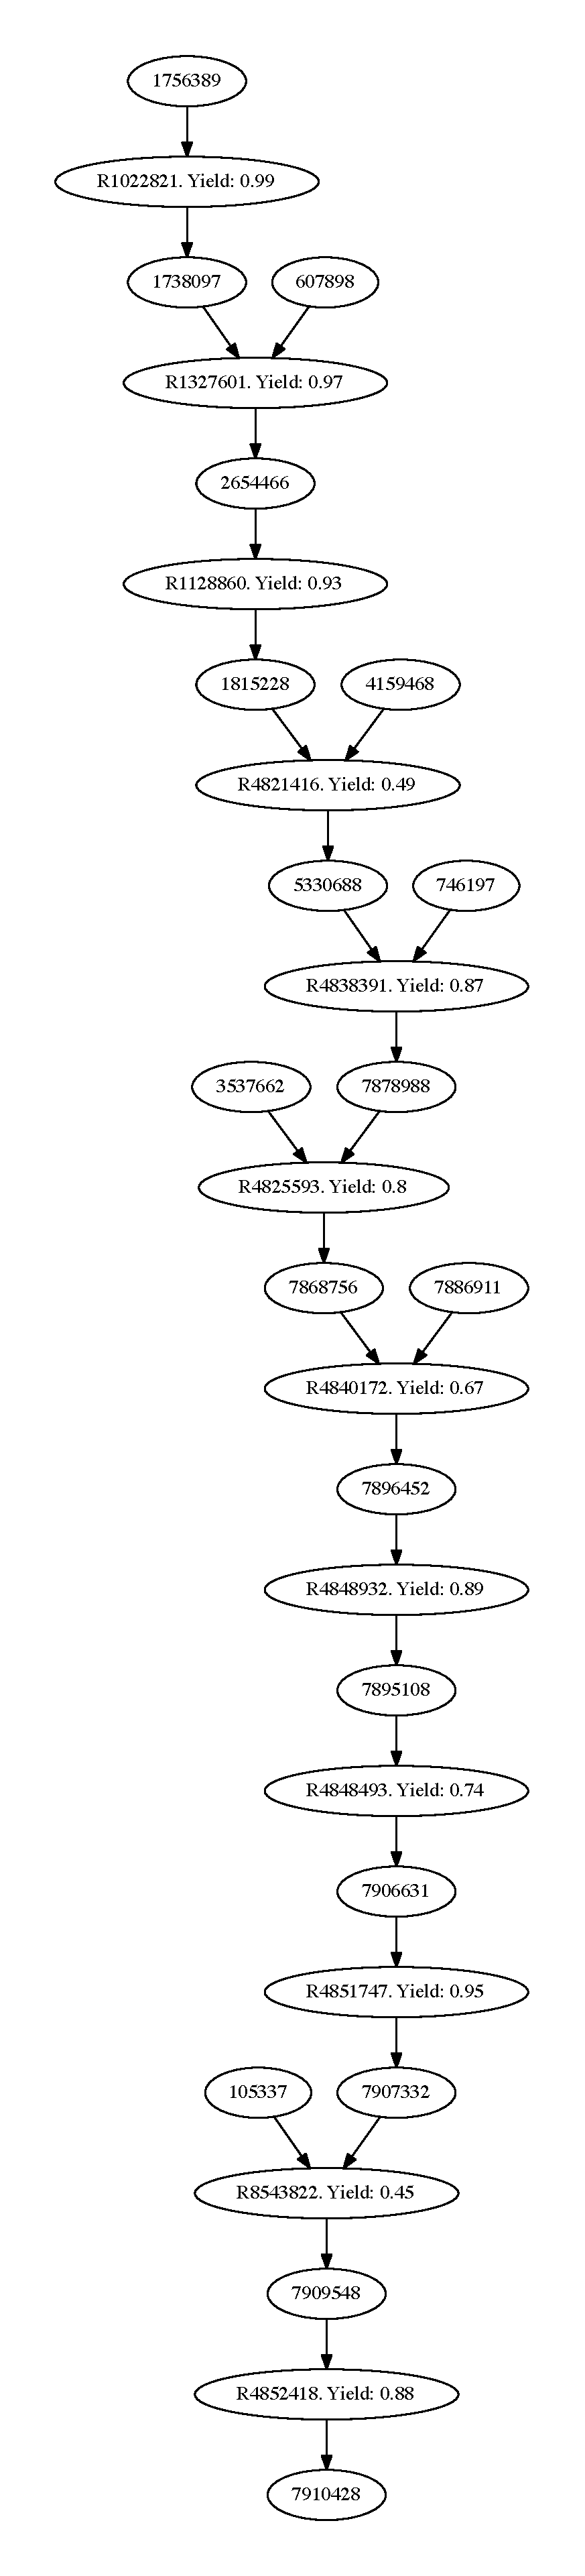
\includegraphics[scale=0.3]{Synteseplaner/Dysidiolide/plan6.pdf}
\label{Appendix::Dysidiolide6}

\subsection{Dysidiolide plan 7}
\centering
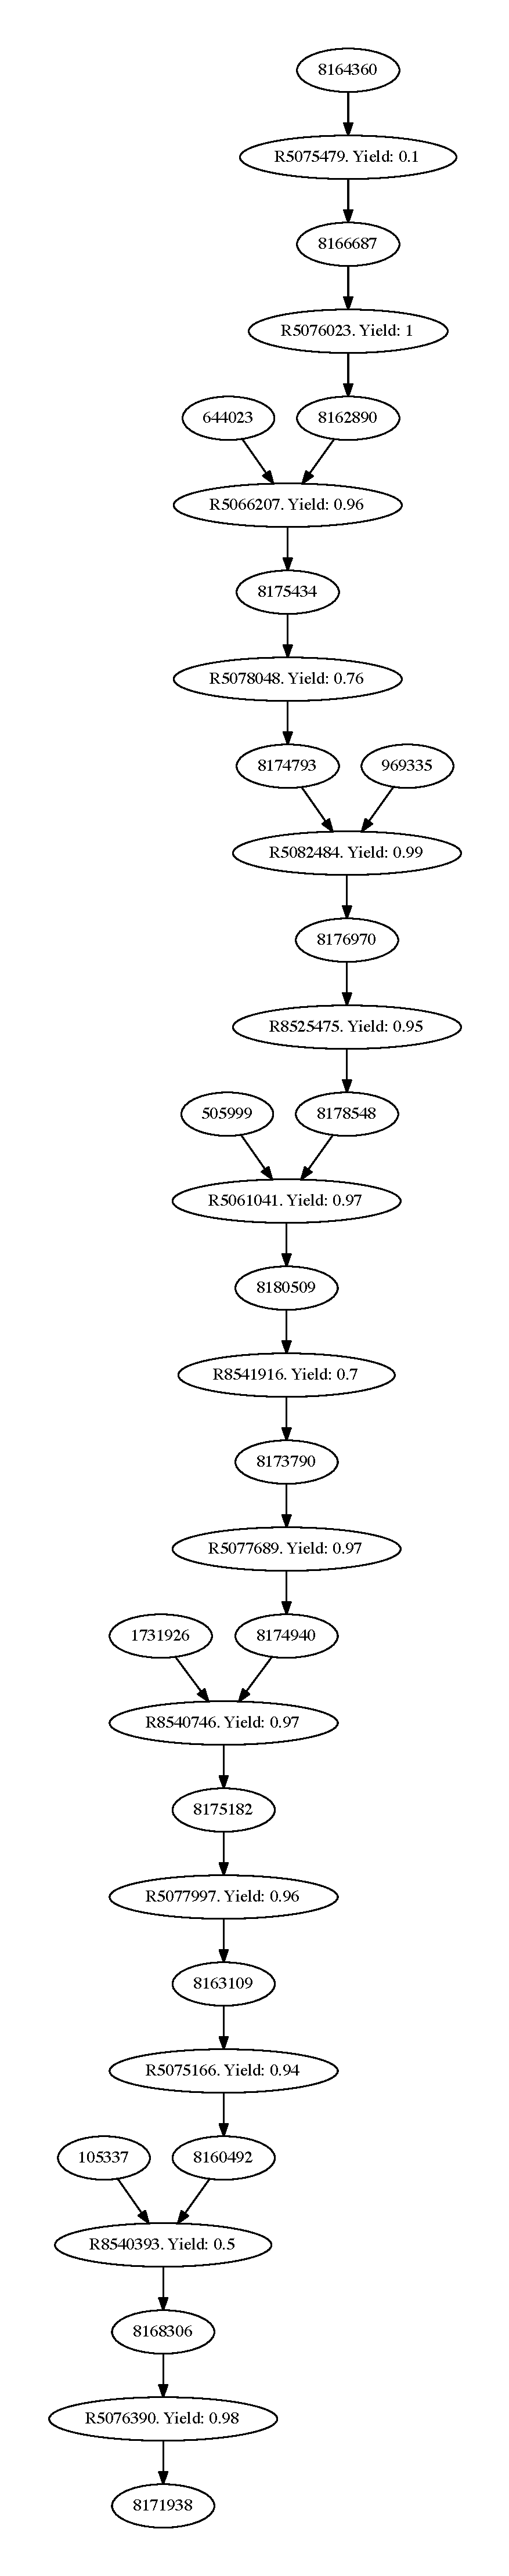
\includegraphics[scale=0.27]{Synteseplaner/Dysidiolide/plan7.pdf}
\label{Appendix::Dysidiolide7}

\subsection{Dysidiolide plan 8}
\centering
\includegraphics[scale=0.2]{Synteseplaner/Dysidiolide/plan8.pdf}
\label{Appendix::Dysidiolide8}

\subsection{Dysidiolide plan 9}
\centering
\includegraphics[scale=0.25]{Synteseplaner/Dysidiolide/plan9.pdf}
\label{Appendix::Dysidiolide9}

\subsection{Dysidiolide plan 10}
\centering
\includegraphics[scale=0.2]{Synteseplaner/Dysidiolide/plan10.pdf}
\label{Appendix::Dysidiolide10}

\subsection{Asteriscanolide plan 1}
\centering
\includegraphics[scale=0.4]{Synteseplaner/Asteriscanolide/plan1.pdf}
\label{Appendix::Asteriscanolide1}

\subsection{Asteriscanolide plan 2}
\centering
\includegraphics[scale=0.4]{Synteseplaner/Asteriscanolide/plan2.pdf}
\label{Appendix::Asteriscanolide2}

\subsection{Asteriscanolide plan 3}
\centering
\includegraphics[scale=0.4]{Synteseplaner/Asteriscanolide/plan3.pdf}
\label{Appendix::Asteriscanolide3}

\subsection{Lepadiformine plan 1}
\centering
\includegraphics[scale=0.4]{Synteseplaner/Lepadiformine/plan1.pdf}
\label{Appendix::Lepadiformine1}

\subsection{Lepadiformine plan 2}
\centering
\includegraphics[scale=0.4]{Synteseplaner/Lepadiformine/plan2.pdf}
\label{Appendix::Lepadiformine2}

\subsection{Lepadiformine plan 3}
\centering
\includegraphics[scale=0.4]{Synteseplaner/Lepadiformine/plan3.pdf}
\label{Appendix::Lepadiformine3}

\subsection{Lepadiformine plan 4}
\centering
\includegraphics[scale=0.4]{Synteseplaner/Lepadiformine/plan4.pdf}
\label{Appendix::Lepadiformine4}

\subsection{Lepadiformine plan 5}
\centering
\includegraphics[scale=0.4]{Synteseplaner/Lepadiformine/plan5.pdf}
\label{Appendix::Lepadiformine5}

\subsection{Lepadiformine plan 6}
\centering
\includegraphics[scale=0.4]{Synteseplaner/Lepadiformine/plan6.pdf}
\label{Appendix::Lepadiformine6}
\end{document}